\ifx\isEmbedded\undefined

\documentclass[12pt]{report}
	
% FONT RELATED
%\usepackage{times} %Move to times font
\usepackage[labelfont=bf,textfont=it]{caption}
\usepackage[utf8]{inputenc}

% LINKS, PAGE OF CONTENT, REF AND CROSS-REF, HEADERS/FOOTERS
\usepackage[hidelinks]{hyperref}
\usepackage{fancyhdr}
\usepackage{acronym}

% FIGURES, GRAPHICS, TABLES
\usepackage{graphicx}
\usepackage{parskip}
%\usepackage{subfigure}
\usepackage{subfig}
\usepackage{wrapfig}
\usepackage{subfloat}

% COLOURS, TEXT AND FORMATTING
\usepackage{array}
\usepackage{color}
\usepackage{setspace}
\usepackage{longtable}
\usepackage{multirow}

% ADVANCED MATHS, PSEUDO-CODE
\usepackage{amsmath}
\usepackage{alltt}
\usepackage{amsfonts}

% BIBLIOGRAPHY
\usepackage[authoryear]{natbib}
\bibpunct{(}{)}{;}{a}{,}{,}

% USE IN DISSER:

\setlength\oddsidemargin{0.85cm}
\setlength\evensidemargin{0.85cm}

\setlength\textheight{21.0cm}
\setlength\textwidth{15.0cm}

% indent at each new paragrapg
\setlength\parindent{0.5cm}

\setlength\topmargin{-0.2in}
\renewcommand{\baselinestretch}{1.3}

%REPORT

%\setlength\oddsidemargin{1cm}
%\setlength\evensidemargin{0.3in}
%%\setlength\headsep{2.5in}
%
%\setlength\textheight{9.0in}
%\setlength\textwidth{5.5in}
%
%% indent at each new paragrapg
%\setlength\parindent{0.5cm}
%
%%\setlength{\parskip}{10.5ex}
%
%\setlength\topmargin{-0.2in}

%\newcommand{\HRule}{\rule{\linewidth}{0.5mm}}
\newcommand{\HRule}{\rule{\linewidth}{0.0mm}}

% Color definitions (RGB model)
\definecolor{ms-comment}{rgb}{0.1, 0.4, 0.1}
\definecolor{ms-question}{rgb}{0.4, 0.0, 0.0}
\definecolor{ms-new}{rgb}{0.2, 0.4, 0.8}


\graphicspath{{../img/}}
\begin{document}
\fi

\chapter{Applications and Results}
\label{chap:applications_and_results}

\section{Possible real production pipeline}

This chapter has much relevance since it exposes all the different behaviours scripted in order to test the core and perform a set of simulations. But before doing that, it is proposed a real pipeline where this thesis may fit in, proving that this approach might contribute both to the game and VFX industry.

\begin{figure}[!htb]
  \centering
  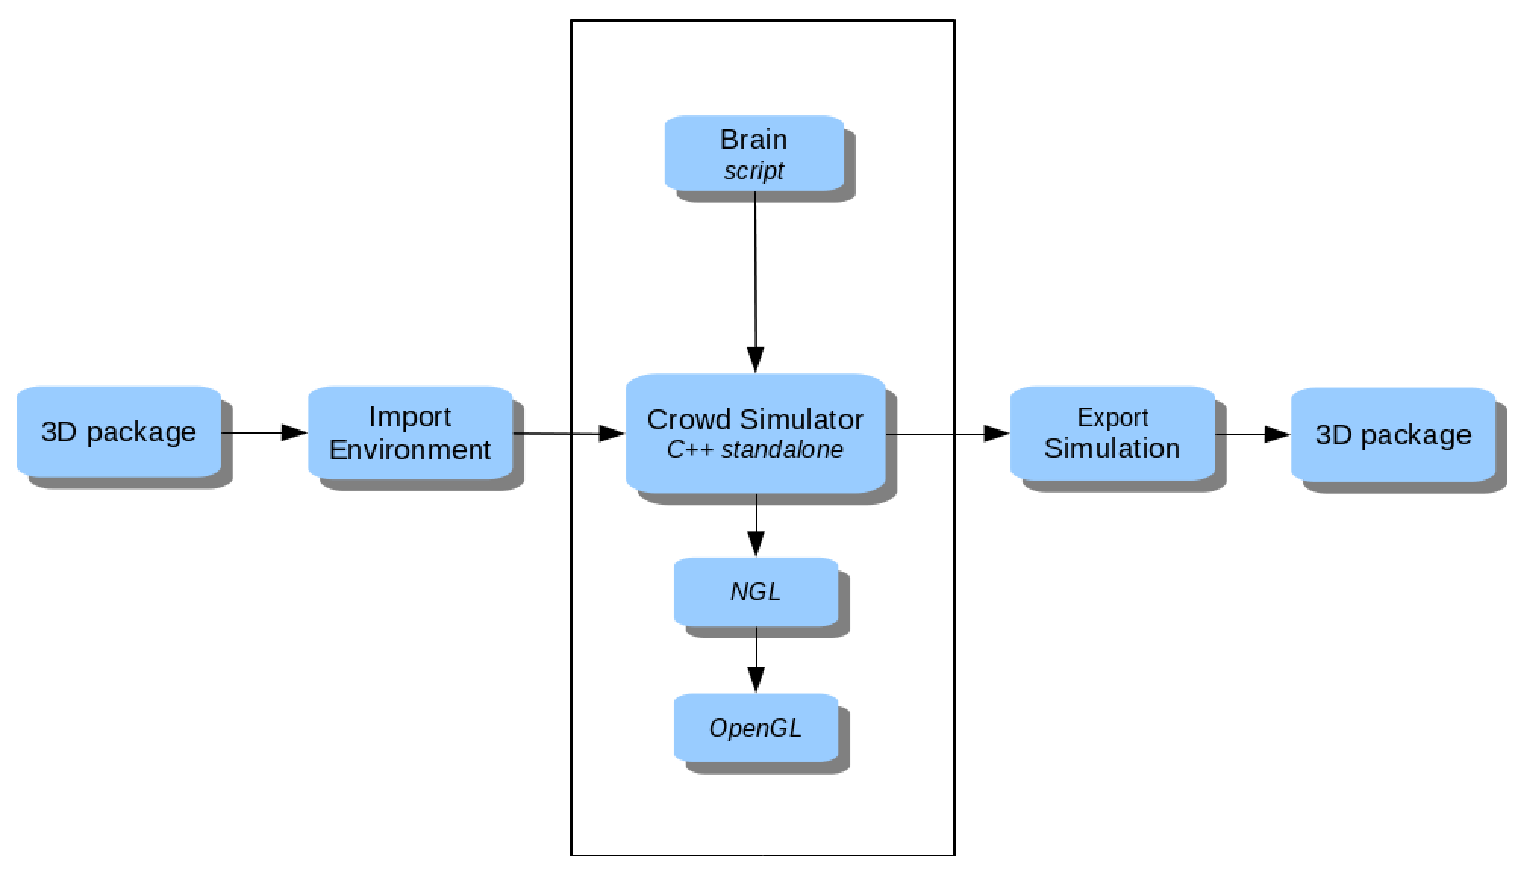
\includegraphics[scale=0.5]{pipeline.eps}
  \caption{Possible pipeline}
  \label{fig:classDiag}
\end{figure}

Any simulation takes place inside a specific environment, therefore it should be possible to import it from a 3D package. When developing this approach, the priorities were behaviours and AI, hence this was left on a second plane. Adding a specific terrain would allow to achieve concrete sequences where a crowd with a particular behaviour is involved.

In order to allow the engine handle the environment, as well as complex meshes for the agents, it would be needed an efficient physics engine able to produce an accurate collision detection. 

Besides of the previous features, the strength of this approach resides in the flexibility of the behaviours. A script-based brain for a new type of agent can be written, modified and added at any time, and the limitations of a behaviour are only set by the behaviour writer. So a tool based on this approach could be used for any sort of sequence.

The simulation might be performed in a user-assisted way, this means that the user could adjust the different parameters that will modify the simulation. The final behaviour emerges from the individual behaviours and their interconnections (this is what this thesis is all about), but as mentioned in the previous chapter, there are physical properties of the virtual world which may lead the simulation in one direction or another.

As final step, the simulation may be exported for finer manipulation and some animations might be attached to each one of the states of the agents.

Another alternative pipeline might be directly build a plugin that can be loaded at runtime by a 3D full package such as Maya or Houdini.

It is worthy to mention that this thesis describes an approach; a robust and solid base where a very flexible, high quality and productive application can be settle on.

\section{Test Behaviours}

Some behaviours were scripted, in this case in Lua, which is the language chosen for this specific implementation. The behaviours are presented following a structure. First the individual behaviours are explained, in company of the FSMs used for their development if there are, and next the emergent behaviours observed are described.

Notice that for the simulations some different dummies are used. They are just that, dummies to make the visualization more friendly and to provide some intuitive clues about the agent's behaviour. But the simulation is about points, transformations and states; and the group behaviour that emerge.

All the videos are available in online platforms or in the master's thesis website.

\subsection{Crowds}

The first test is very basic. The brain of these agents implements the basic behaviour of a flock described by Reynolds \citep{reynolds}. Here, the boids move on the ground as a group of flocks kept in union by the three basic rules. So, having different flocks interacting in the same region, it is possible to distinguish if a boid belongs to one flock or another. The behaviour emerged here is similiar to the one achieved when used field of forces of navigational mechanisms.

Many different situations might arise when there is contact among several flocks. They might adjust their directions to converge in one big mass of people, they might move parallel in opposite directions, they might diverge, etc.

\begin{figure}[!h]
  \centering
  \begin{tabular}{c c}
  	\subfloat[Random crowd]{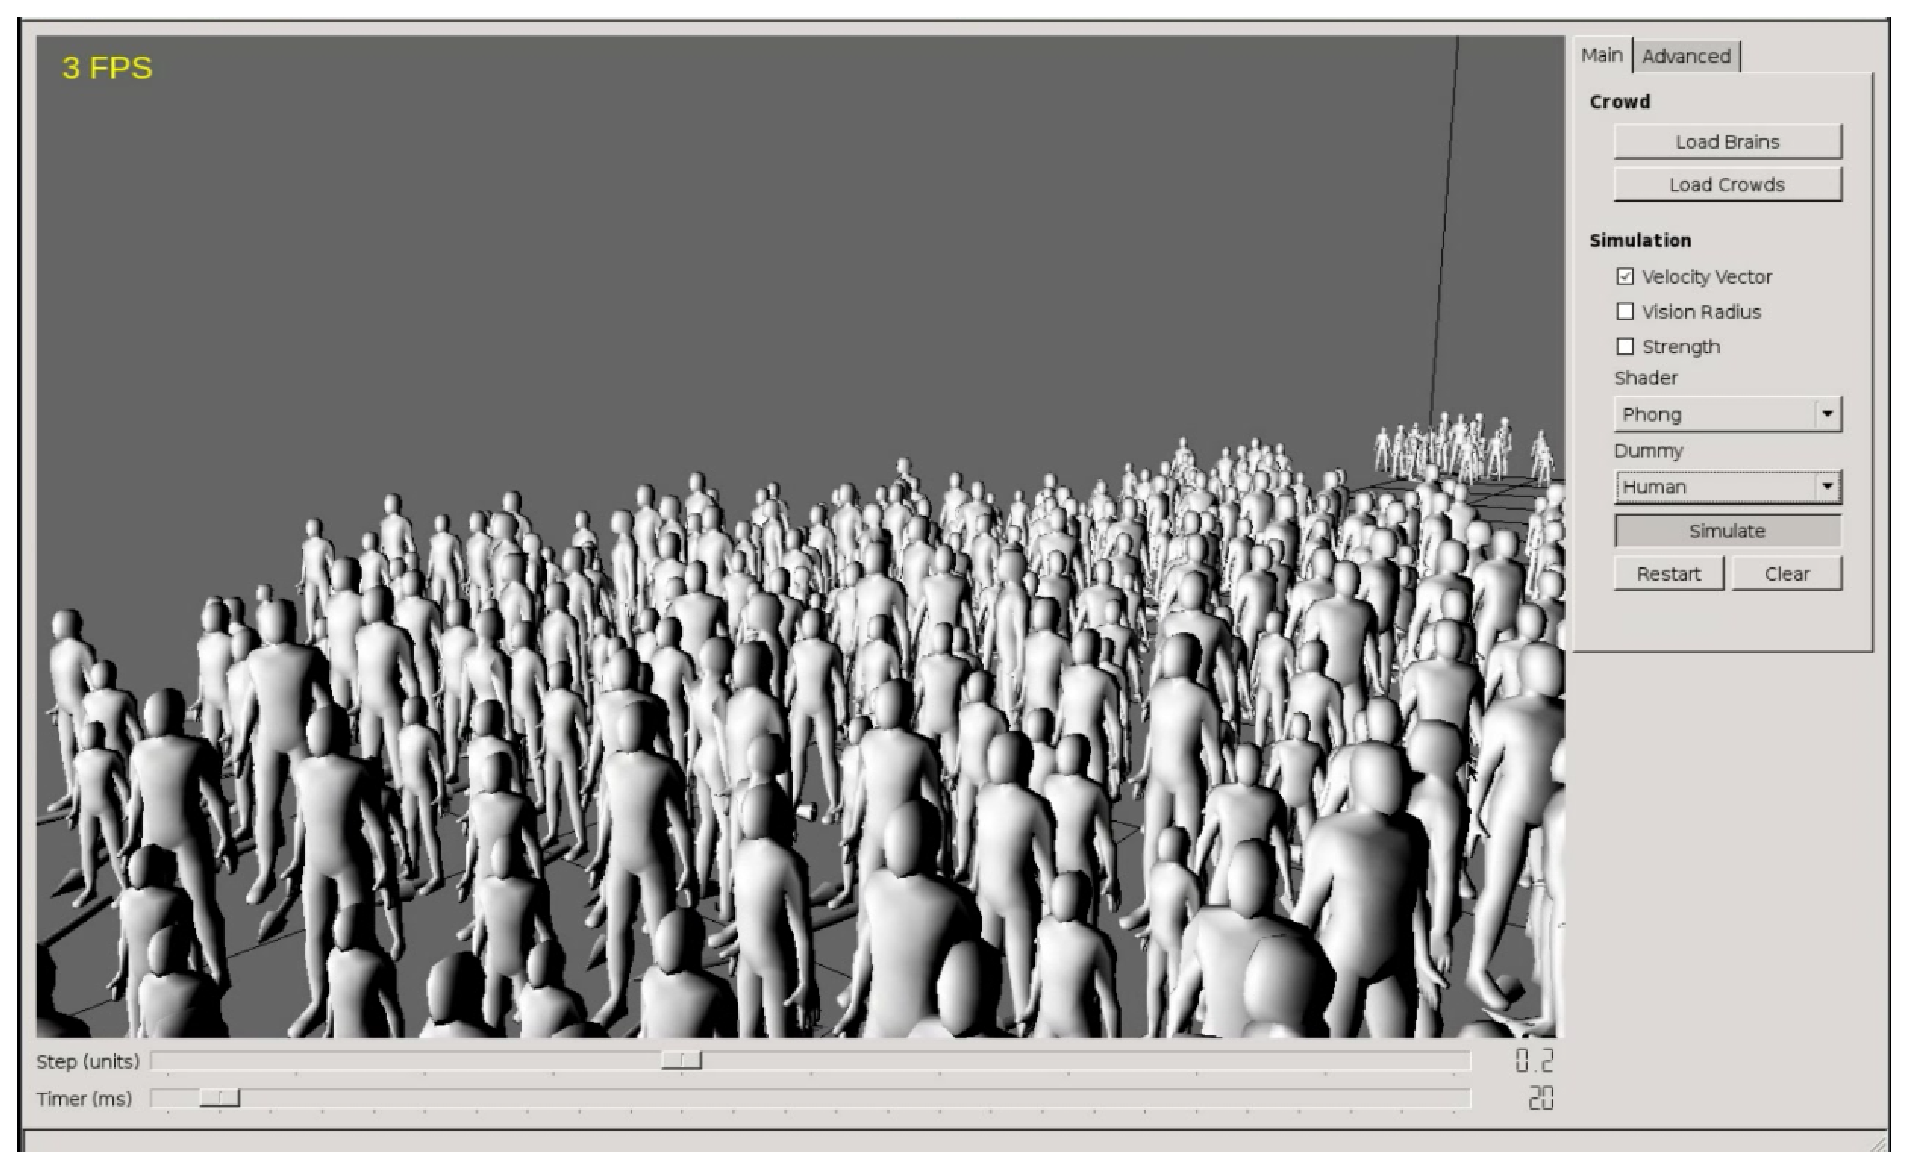
\includegraphics[scale=0.23]{crowds_01.eps}} &
 	\subfloat[Diverging crowd]{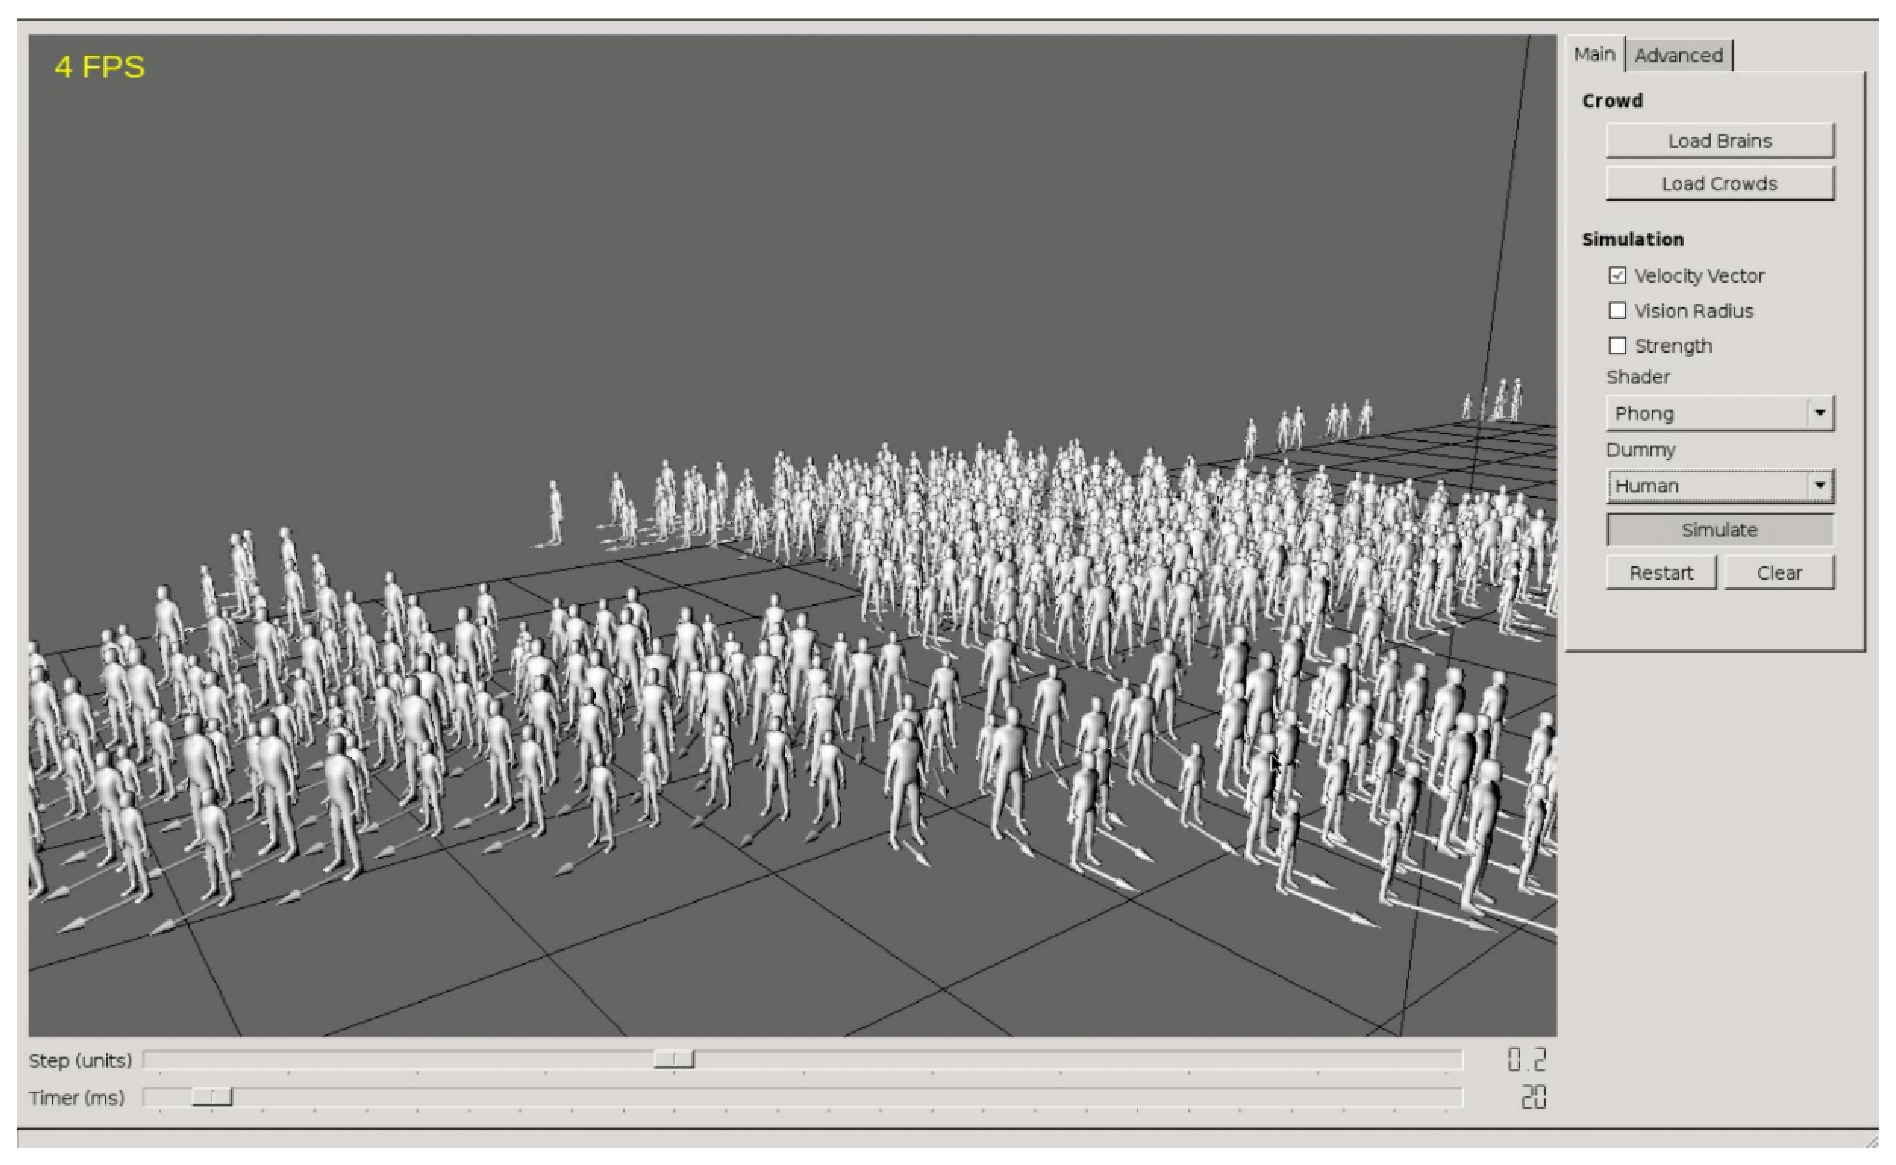
\includegraphics[scale=0.23]{crowds_02.eps}} \\
 \end{tabular}
  \caption{Crowd Simulation}
  \label{fig:crowdsCaptures}
\end{figure}

\newpage
\subsection{Droid Wars}

This behaviour is a little more complex than the previous one. The brain reproduces how a \emph{shooter battle droid} acts. 

\begin{figure}[!h]
  \centering
 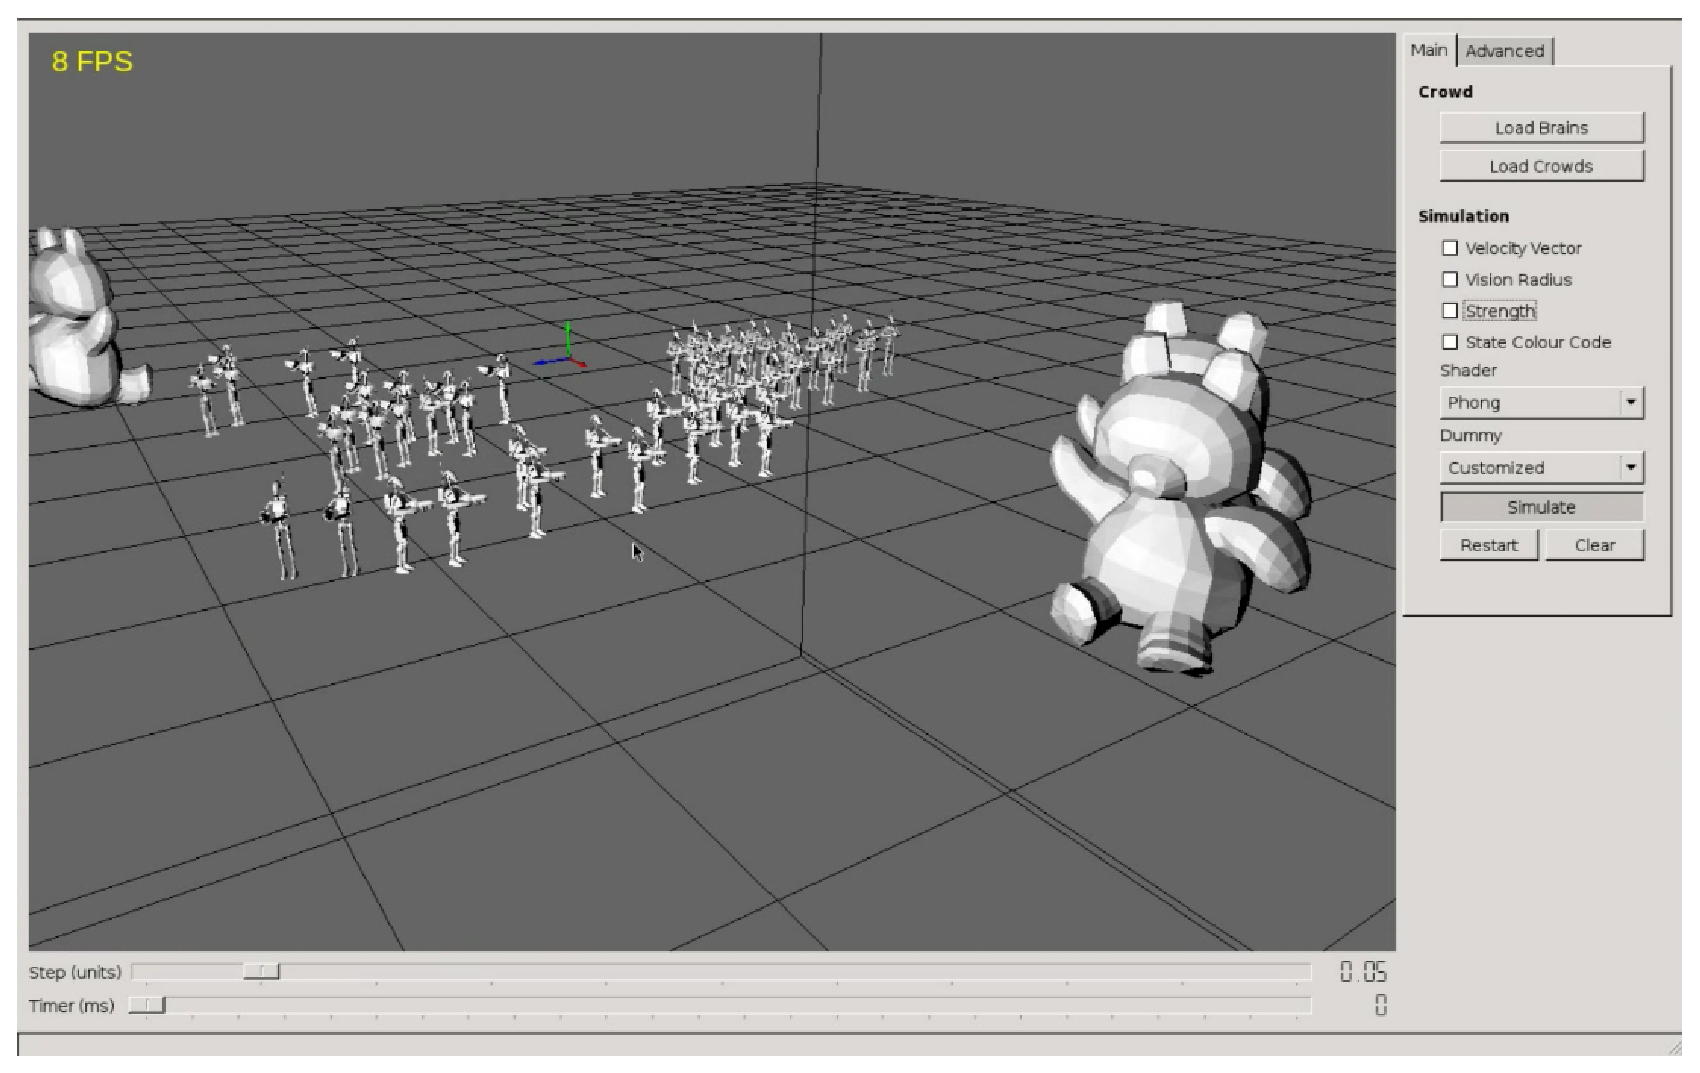
\includegraphics[scale=0.5]{droids_01.eps}
  \caption{Droids and targets}
\end{figure}

They patrol in flocks (green state), so that means that the three Reynolds' flocking algorithm rules are present here too (and in most behaviours). In the simulation, there are also some targets which move randomly on the ground. When a droid sights a target (it enters in its vision radius), it changes of state and starts attacking (red state). Targets receive the shots as messages and they decrease their strength. If a target gets too close to a droid, the droid permutes to a state of evasion to reach a proper distance to shot again (blue state). The FSM is presented below.

\begin{figure}[!h]
  \centering
 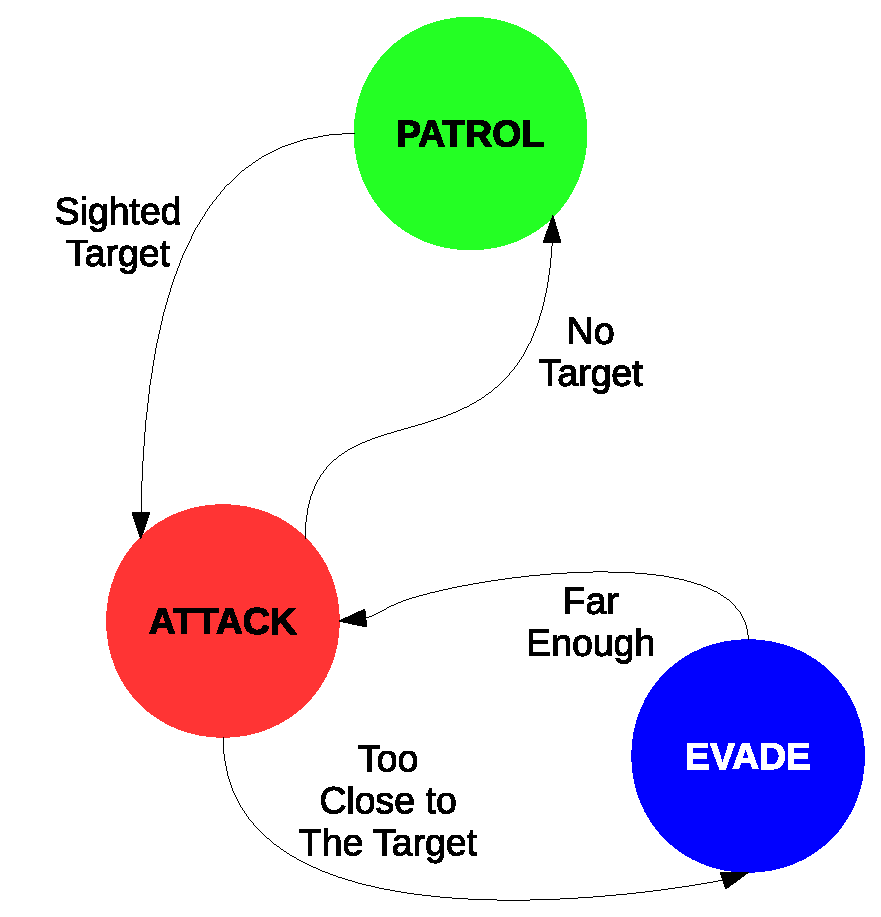
\includegraphics[scale=0.35]{droidFSM.eps}
  \caption{Droid's FSM}
\end{figure}

In the next screen captures it can be observed the group behaviour that arises. They stay at certain distance and attack together, tending to describe arcs around the target. Even if the attack state does not implement the flocking behaviour they group due to common targets.

\begin{figure}[!h]
  \centering
  \begin{tabular}{c c}
  	\subfloat[Droids flocks attacking targets]{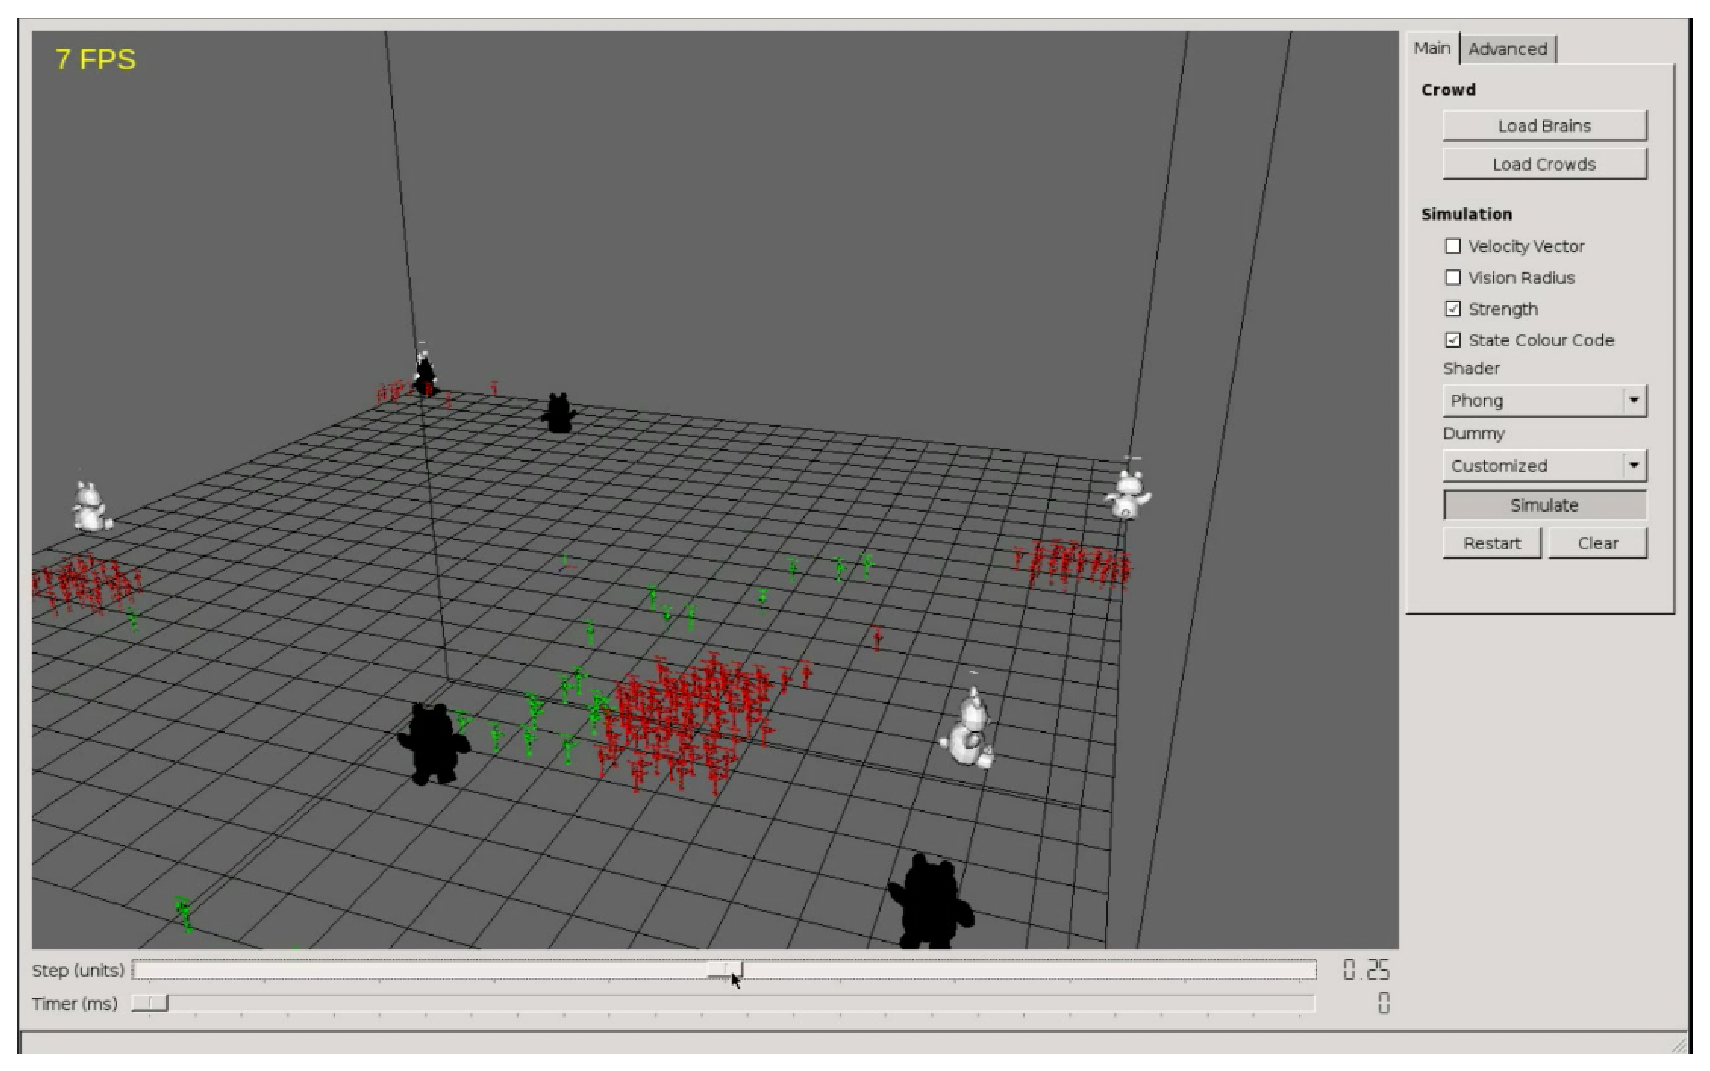
\includegraphics[scale=0.24]{droids_02.eps}} &
 	\subfloat[Droids evading]{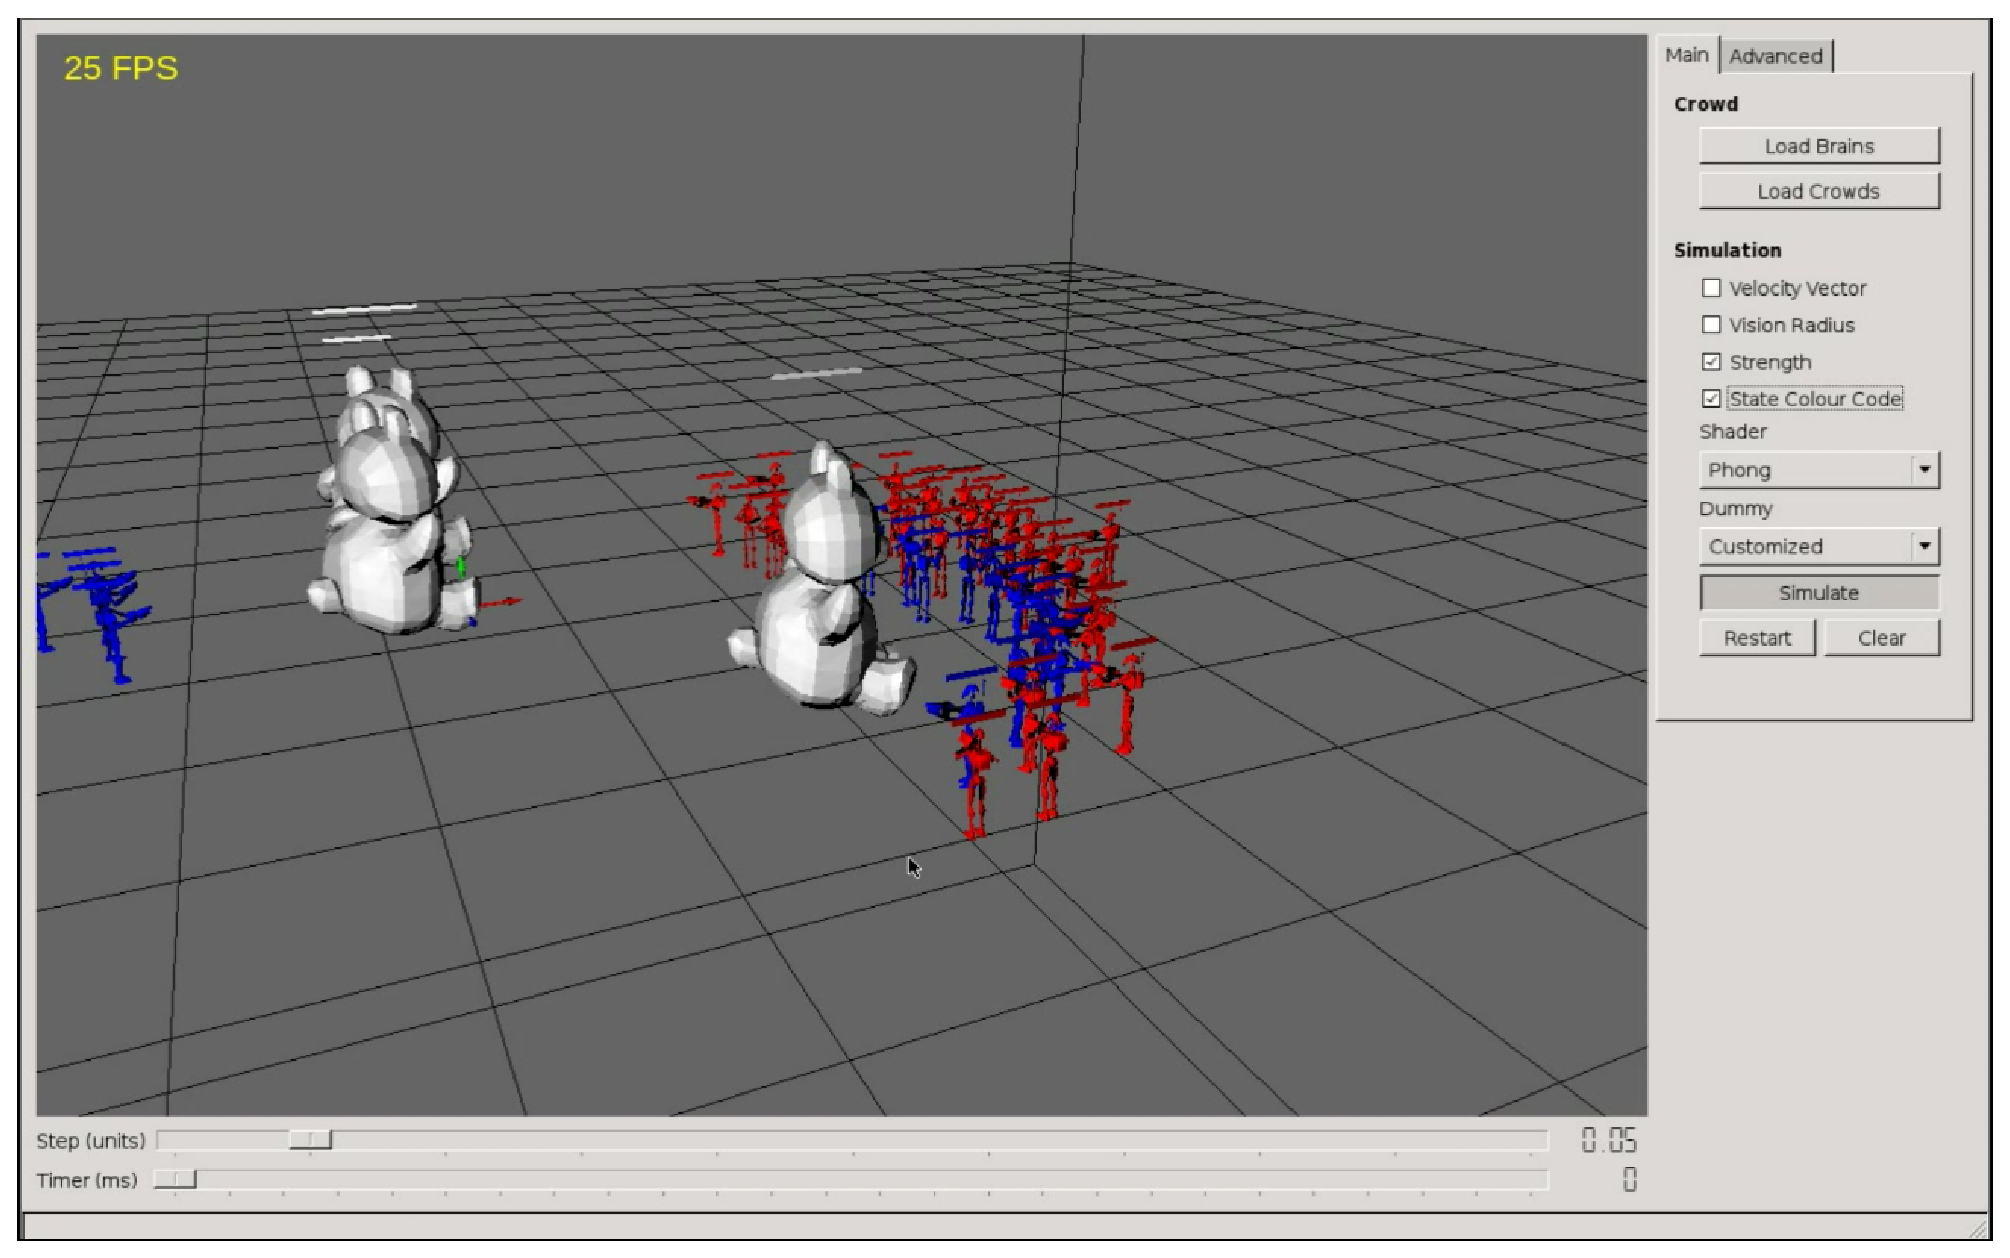
\includegraphics[scale=0.2]{droids_03.eps}} \\
 \end{tabular}
  \caption{Droids War Simulation}
\end{figure}

\subsection{Zombie Apocalypse}

This brain is the less complex one. This is quite logical if we take into account that we are trying to represent zombies. It is just an obsessive behaviour which launches the agent against the \emph{wall}, trying to reach a target point by any mean.  

\begin{figure}[!h]
  \centering
  \begin{tabular}{c c}
  	\subfloat[Obsessive zombies running to the wall]{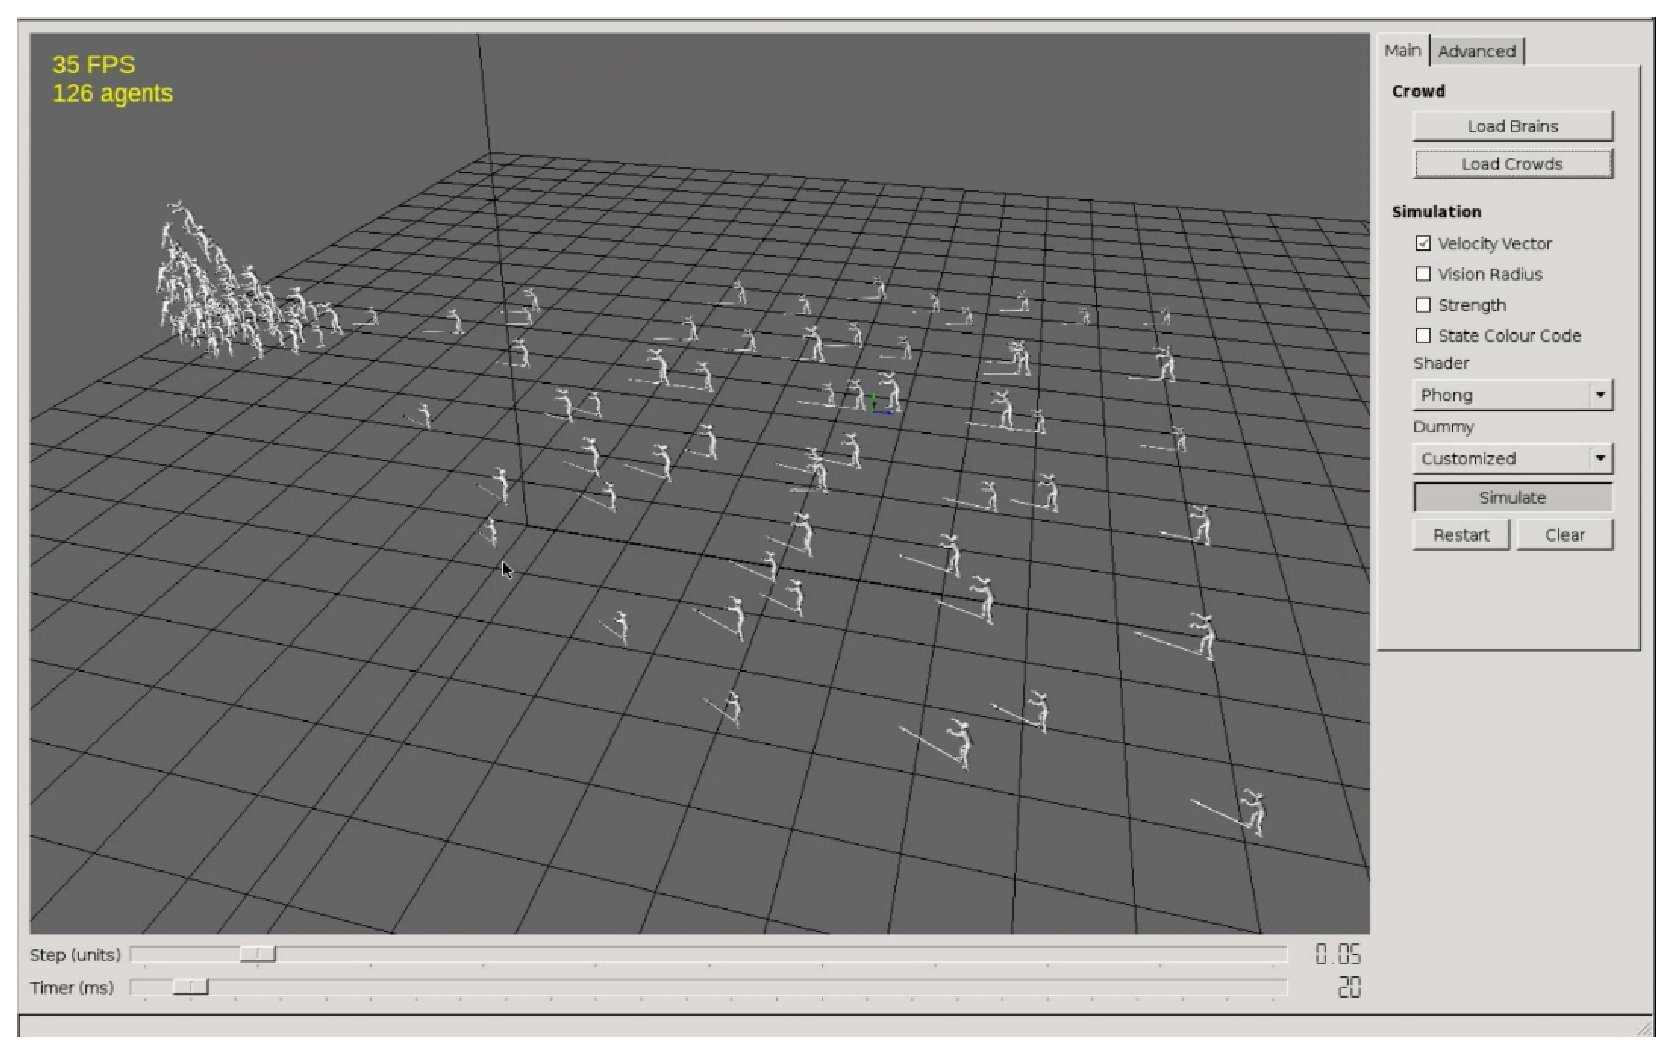
\includegraphics[scale=0.25]{zombies_01.eps}} &
 	\subfloat[Zombies climbing to the wall]{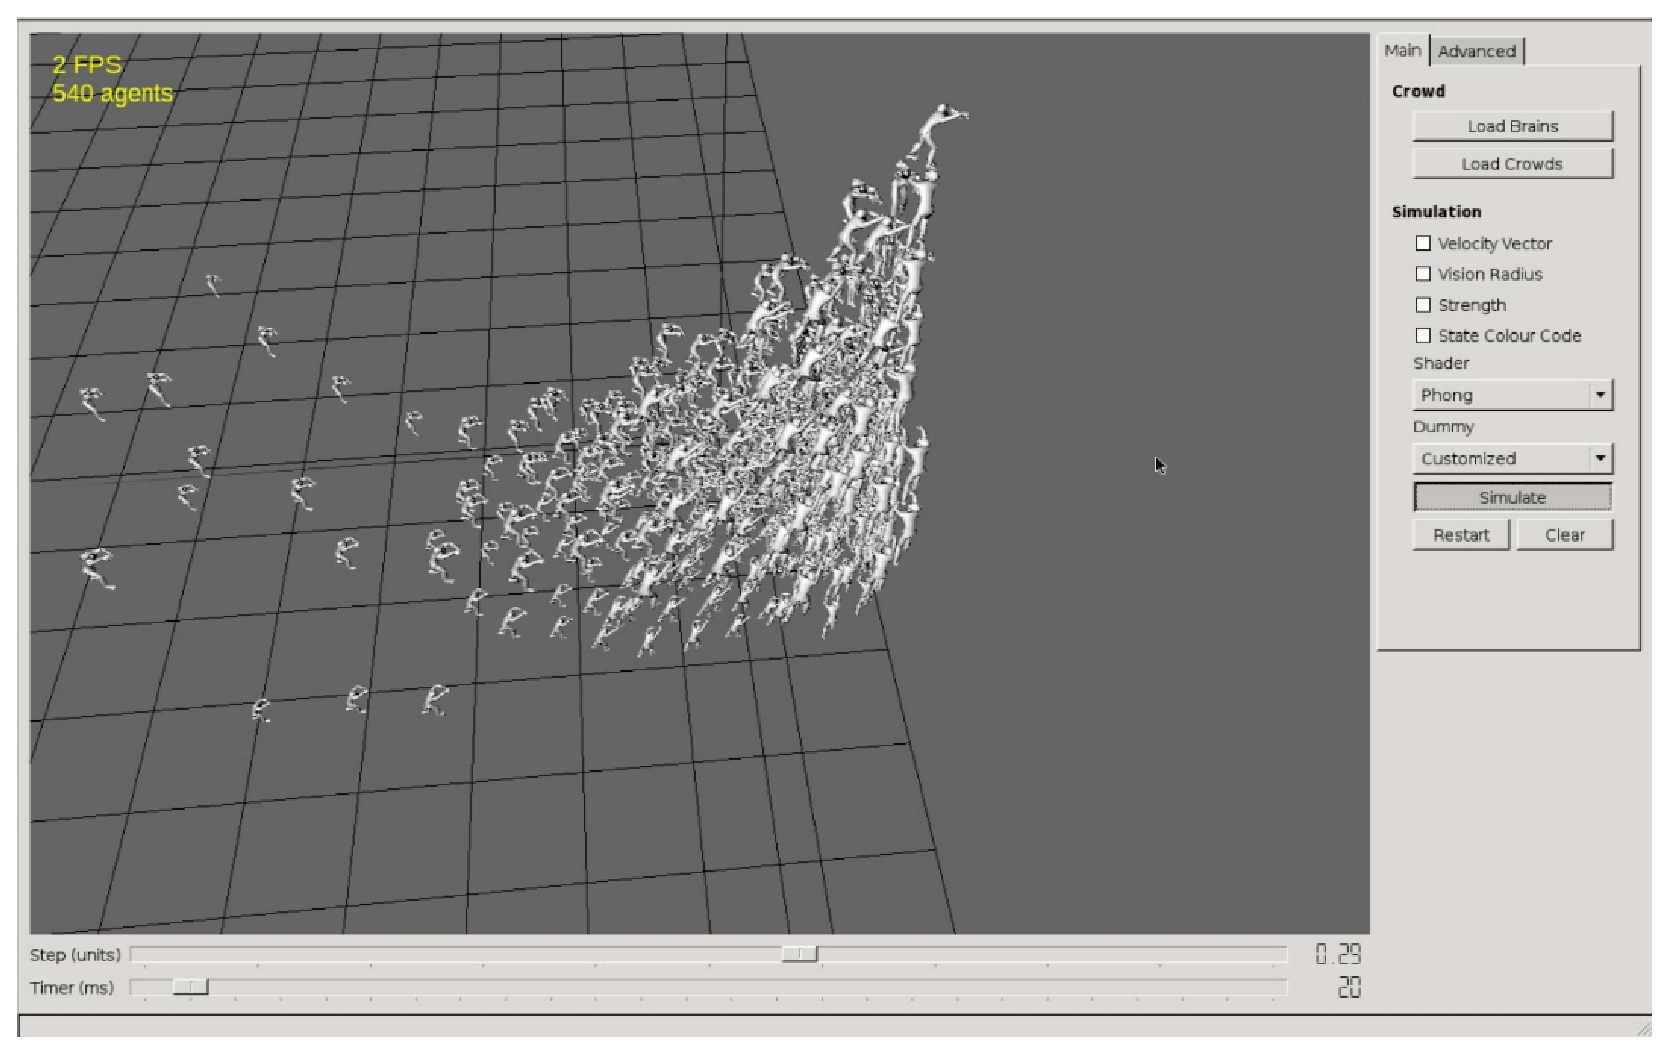
\includegraphics[scale=0.25]{zombies_02.eps}} \\
 \end{tabular}
  \caption{Zombie Apocalypse Simulation}
  \label{fig:zombieCaptures}
\end{figure}

What does the work in here is the sphere-based physics engine, which projects the velocity over the tangent to the spheres. This allows that bigger agents climb onto smaller ones. With a simulation with a number of agents large enough, the behaviour that emerges corresponds to a group of not too smart agents, climbing on one another to desperately reach their target, creating a huge human mountain.

\begin{figure}[!h]
  \centering
	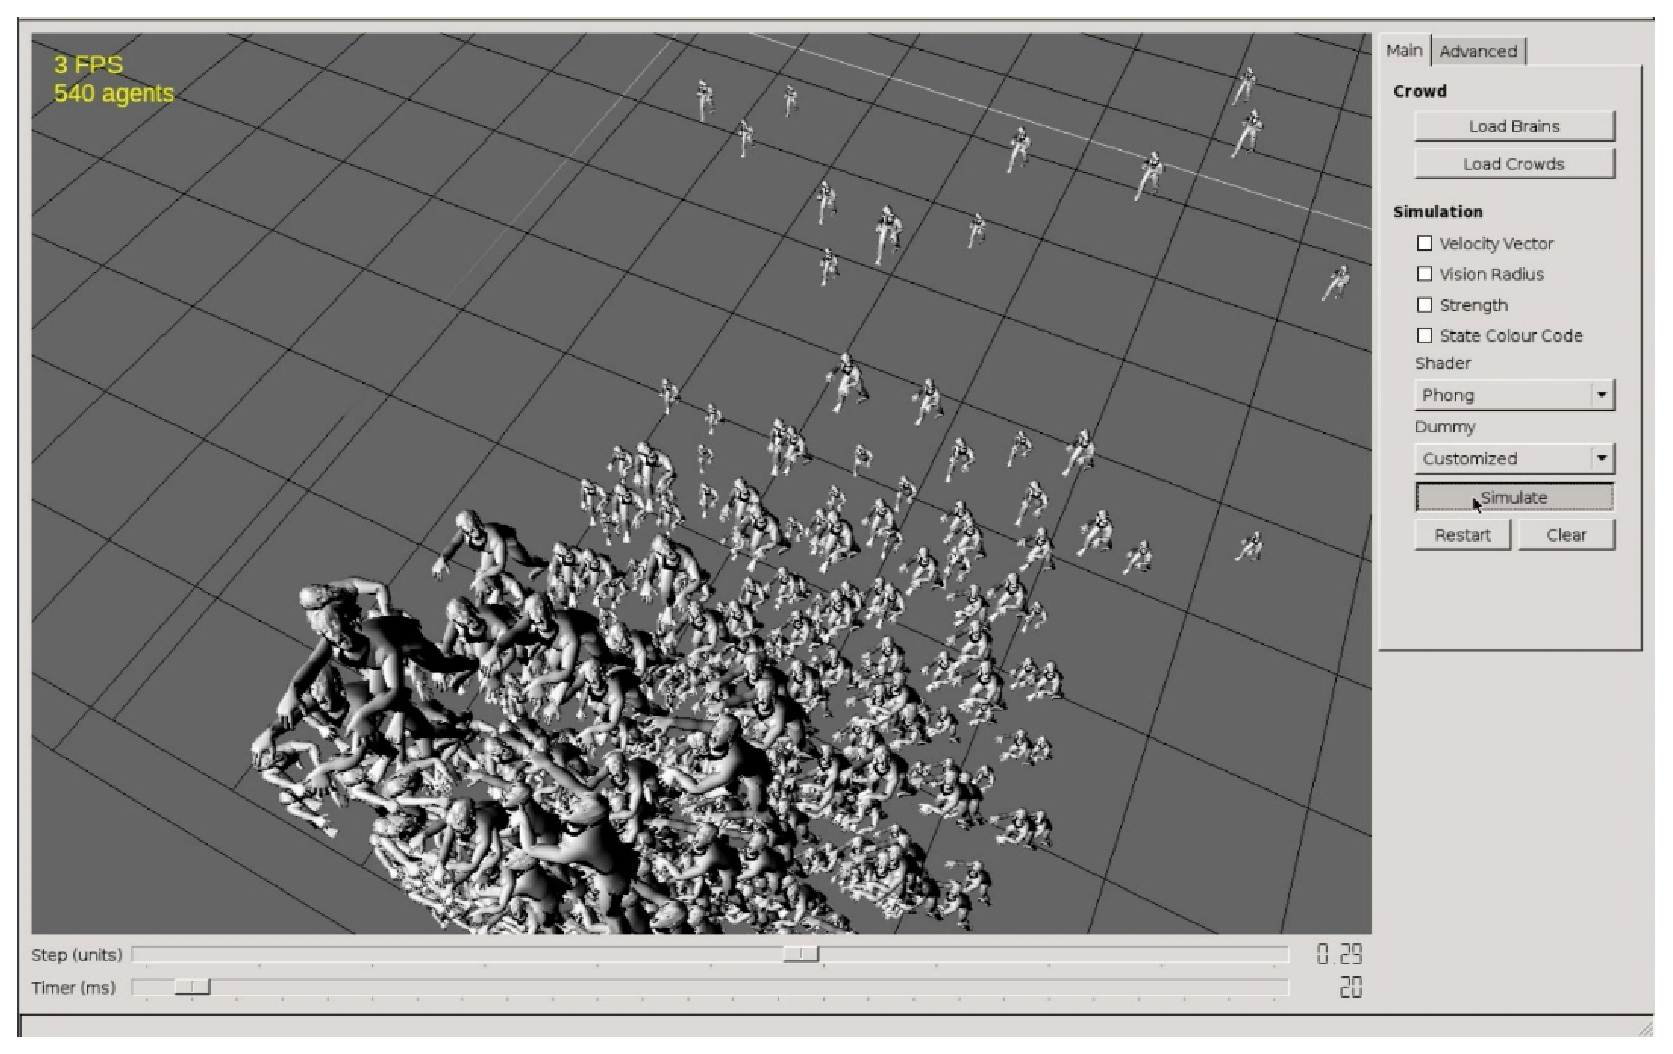
\includegraphics[scale=0.5]{zombies_03.eps}
	\caption{Mountain of zombies}
  \label{fig:zombieCaptures}
\end{figure}

\newpage
\subsection{A Battlefield}

This example might be the more complete one, it includes several behaviours with different characteristics that, by means of message passing, can communicate among all of them. The \emph{warrior} brain, is the classical member of a battle. It moves with their troop and when it sights an enemy it attacks it. Contrary to the shooter behaviour, this is a body-to-body fight so a warrior can send attacks to the enemy stepping forward, or receive attacks having to step back. If the strength is too critical, the warrior switches to a state of defense, sending no attack and recovering strength. The FSM is presented below.

\begin{figure}[!h]
  \centering
 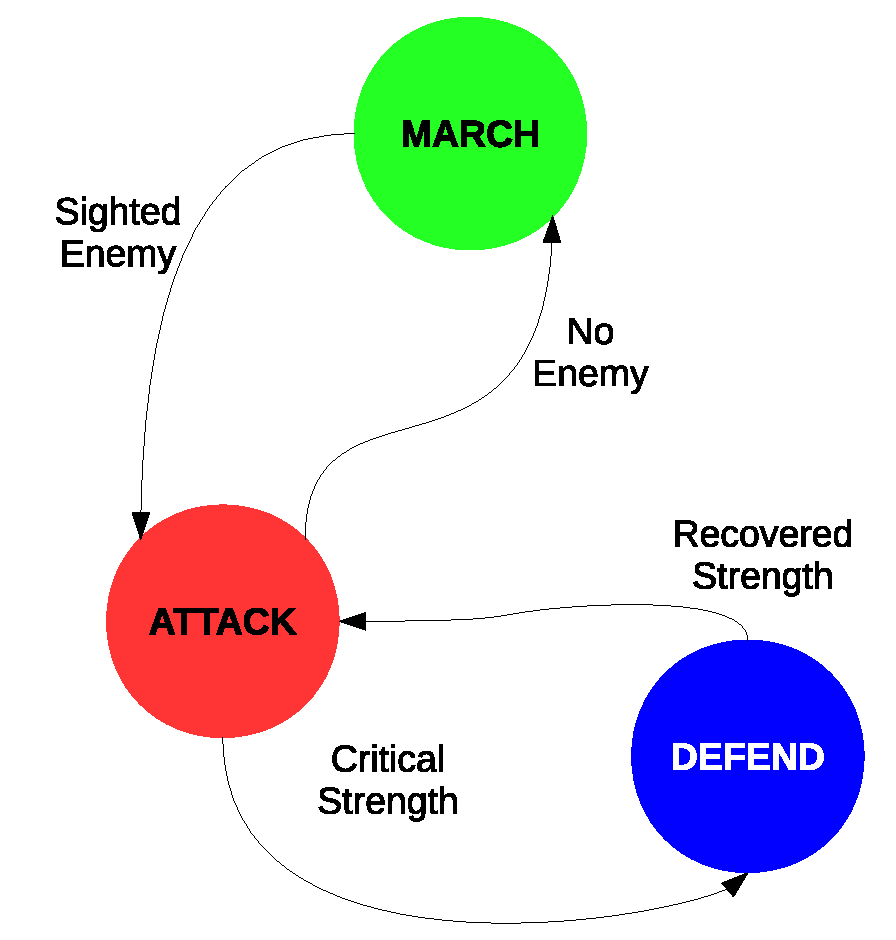
\includegraphics[scale=0.35]{warriorFSM.eps}
  \caption{Warrior's FSM}
\end{figure}

In the same way, it was developed a very similar brain to the warrior called \emph{captain}. The captain commands warriors and has to lead the troop to the enemy. Thus, he has extra movement freedom besides the flocking properties. It is similar to a leader boid.

The emergent behaviours that may arise in this situations are infinite. Normally, after the clash of two armies, warriors will start to join in small groups, such as couples or three or four, fighting among them. Warriors that do not sight the enemy will march together where, although the movement may be highly synchronous, their physical properties will condition their march.

\begin{figure}[!h]
  \centering
  \begin{tabular}{c c}
  	\subfloat[Fighting behaviours]{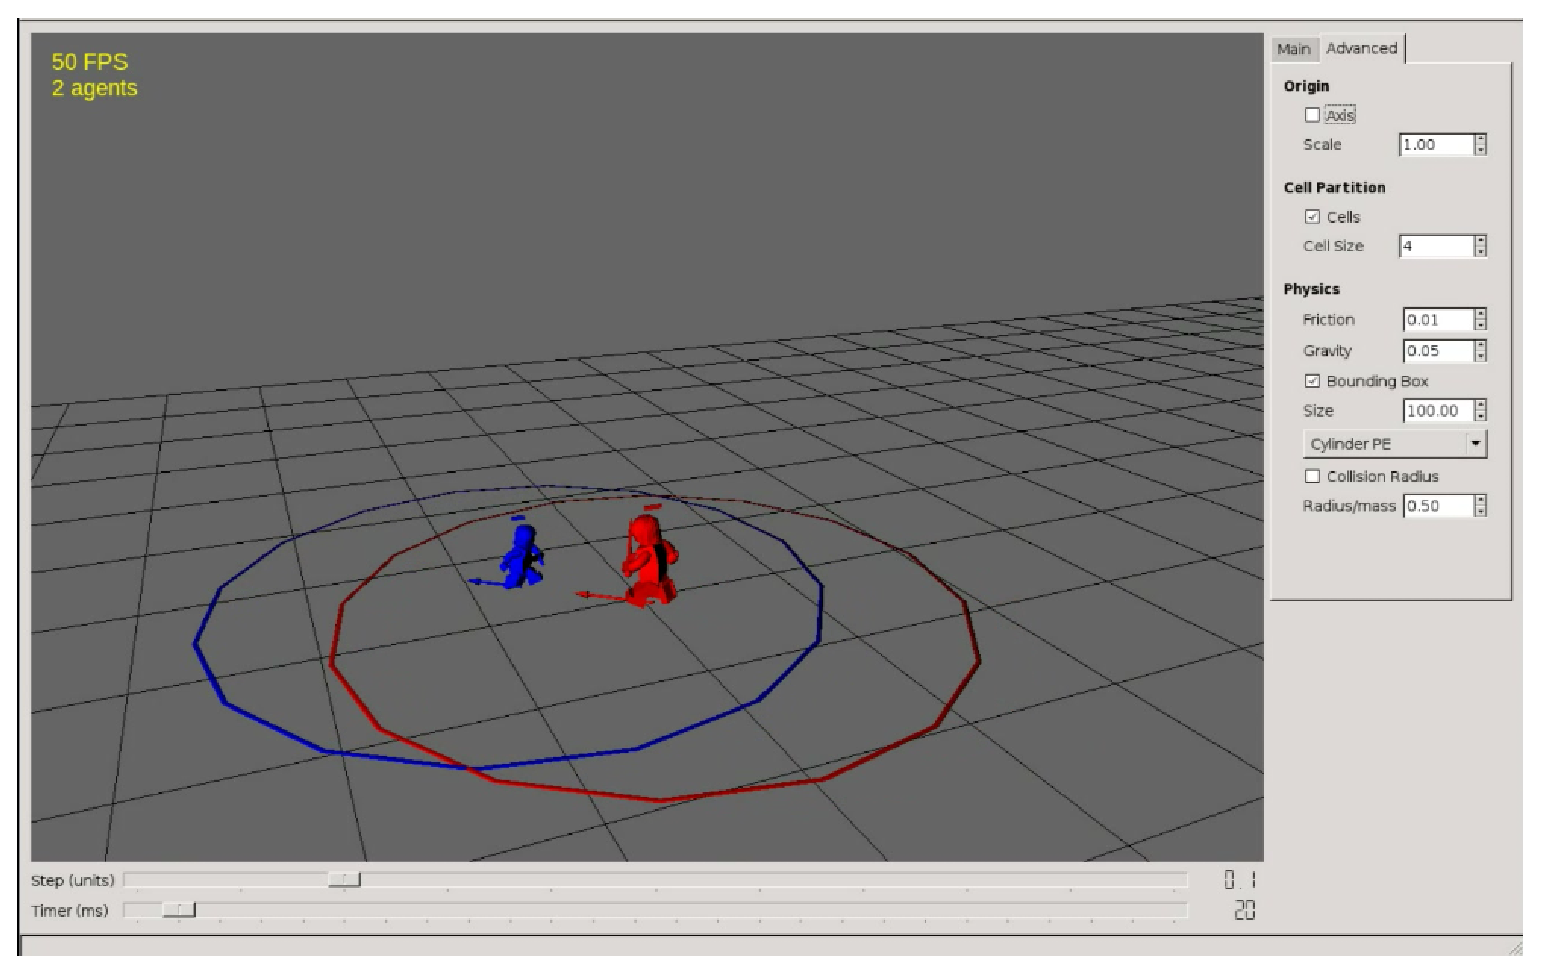
\includegraphics[scale=0.28]{battle_01.eps}} &
 	\subfloat[Sparse battlefield]{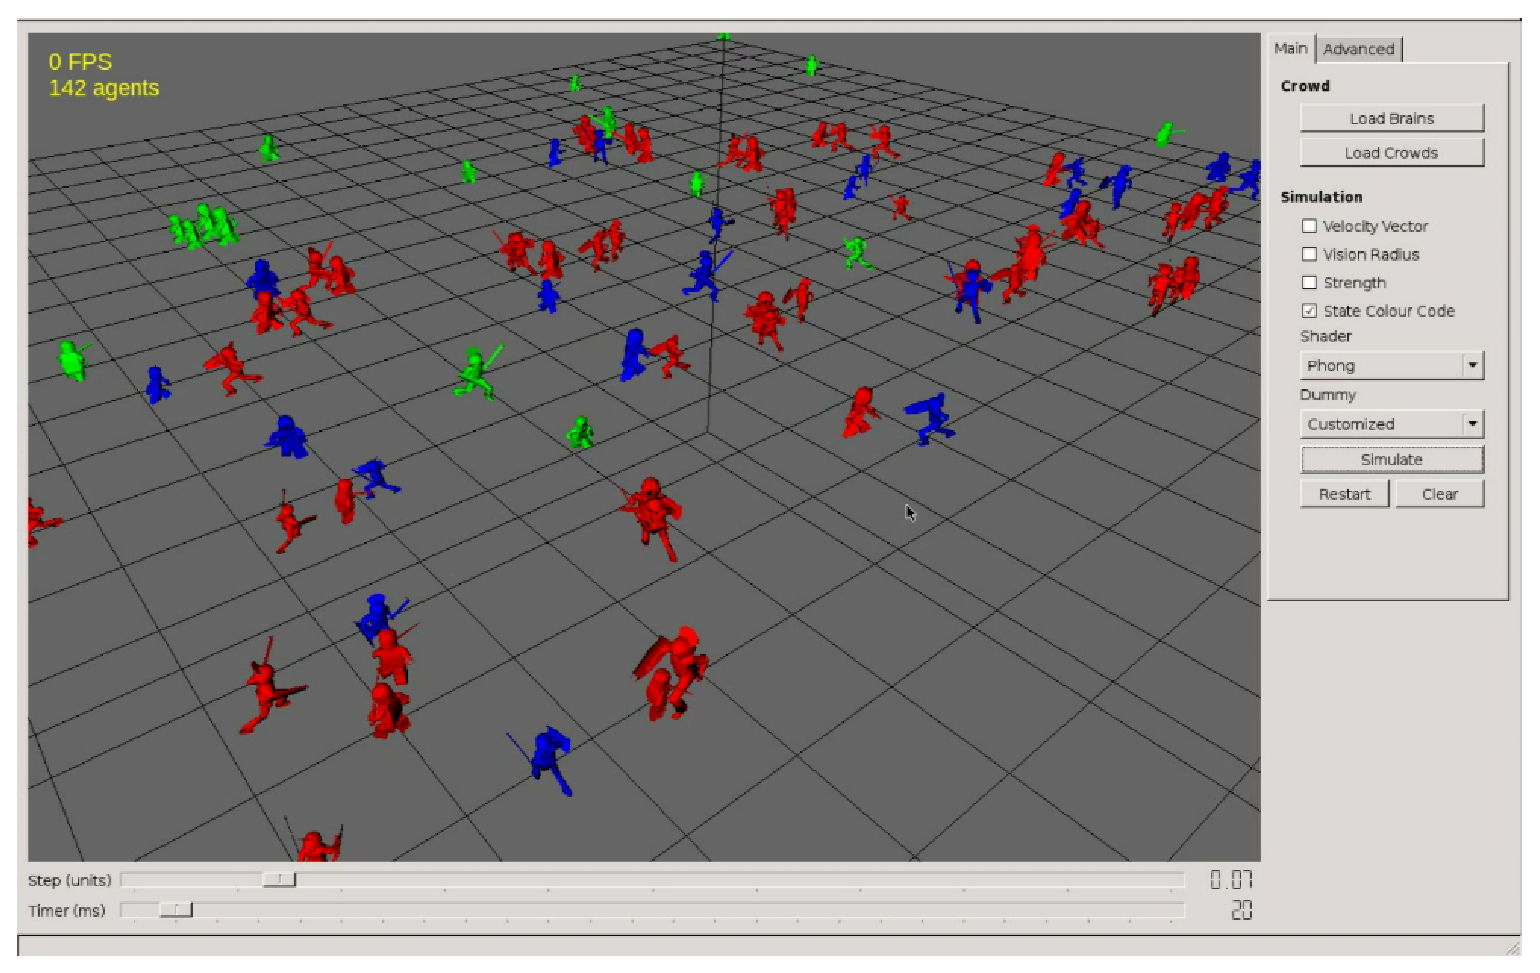
\includegraphics[scale=0.28]{battle_02.eps}} \\
 	\subfloat[Dense battlefield]{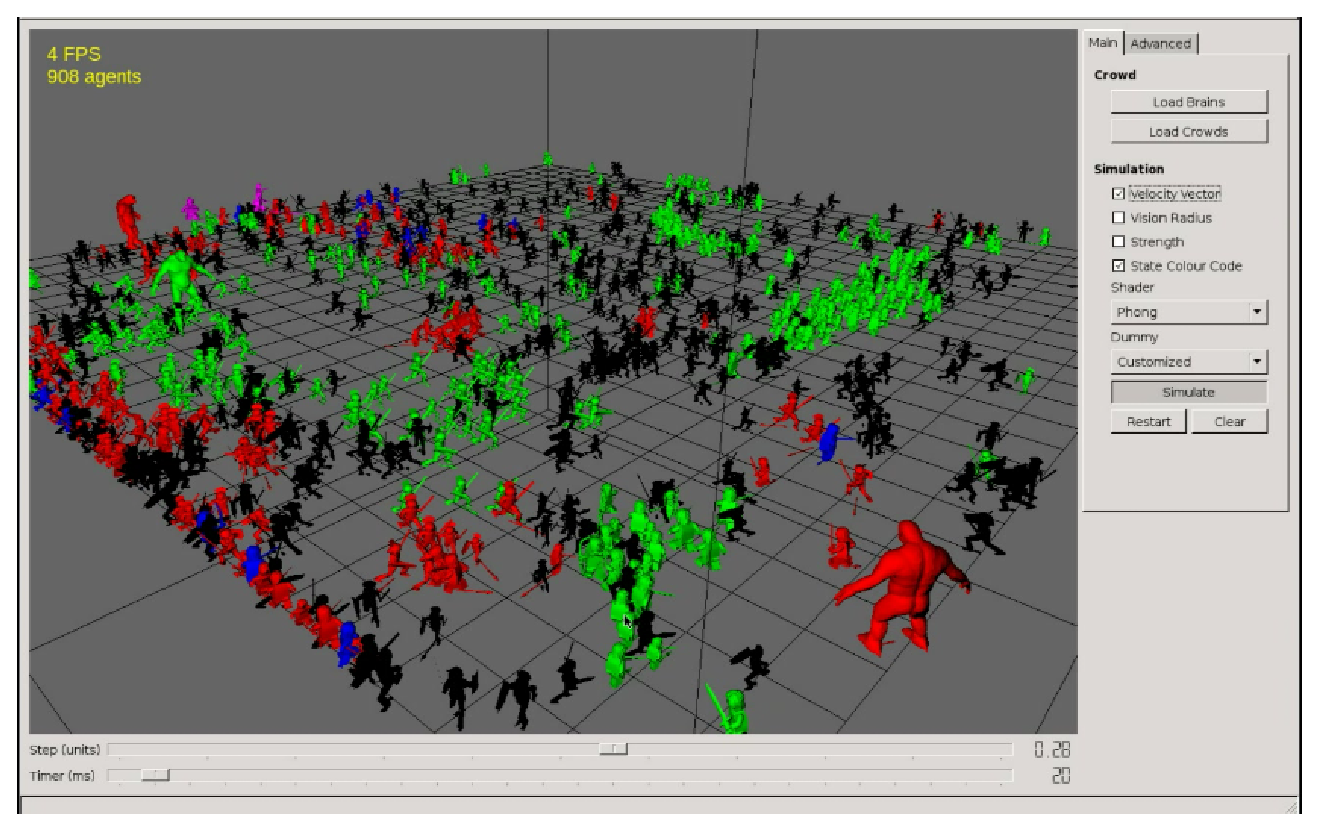
\includegraphics[scale=0.33]{battle_03.eps}} &
 	\subfloat[Marching troops]{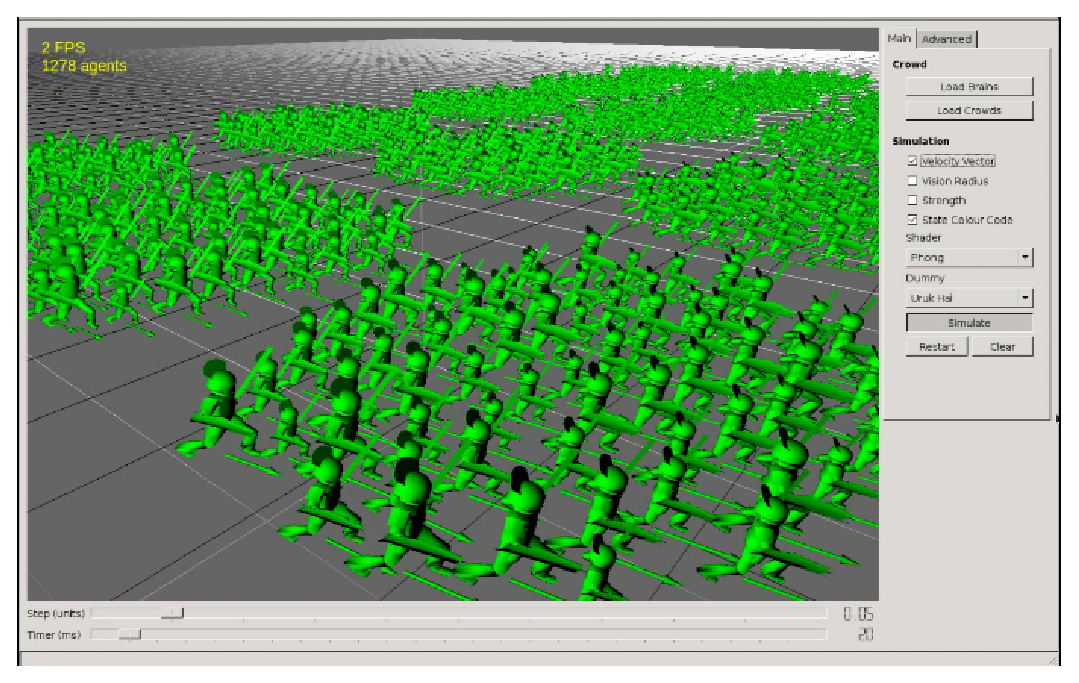
\includegraphics[scale=0.4]{battle_04.eps}} \\
 \end{tabular}
  \caption{A Battlefield Simulation}
  \label{fig:battleCaptures}
\end{figure}

In order to enrich the battlefield, some extra behaviours were also developed. The \emph{archer} brain is very similar to the shooter droid, and the \emph{troll}, although slower, is capable to apply attacks much stronger than a current warrior.

\begin{figure}[!h]
  \centering
  \begin{tabular}{c c}
  	\subfloat[Flock of archer behaviours]{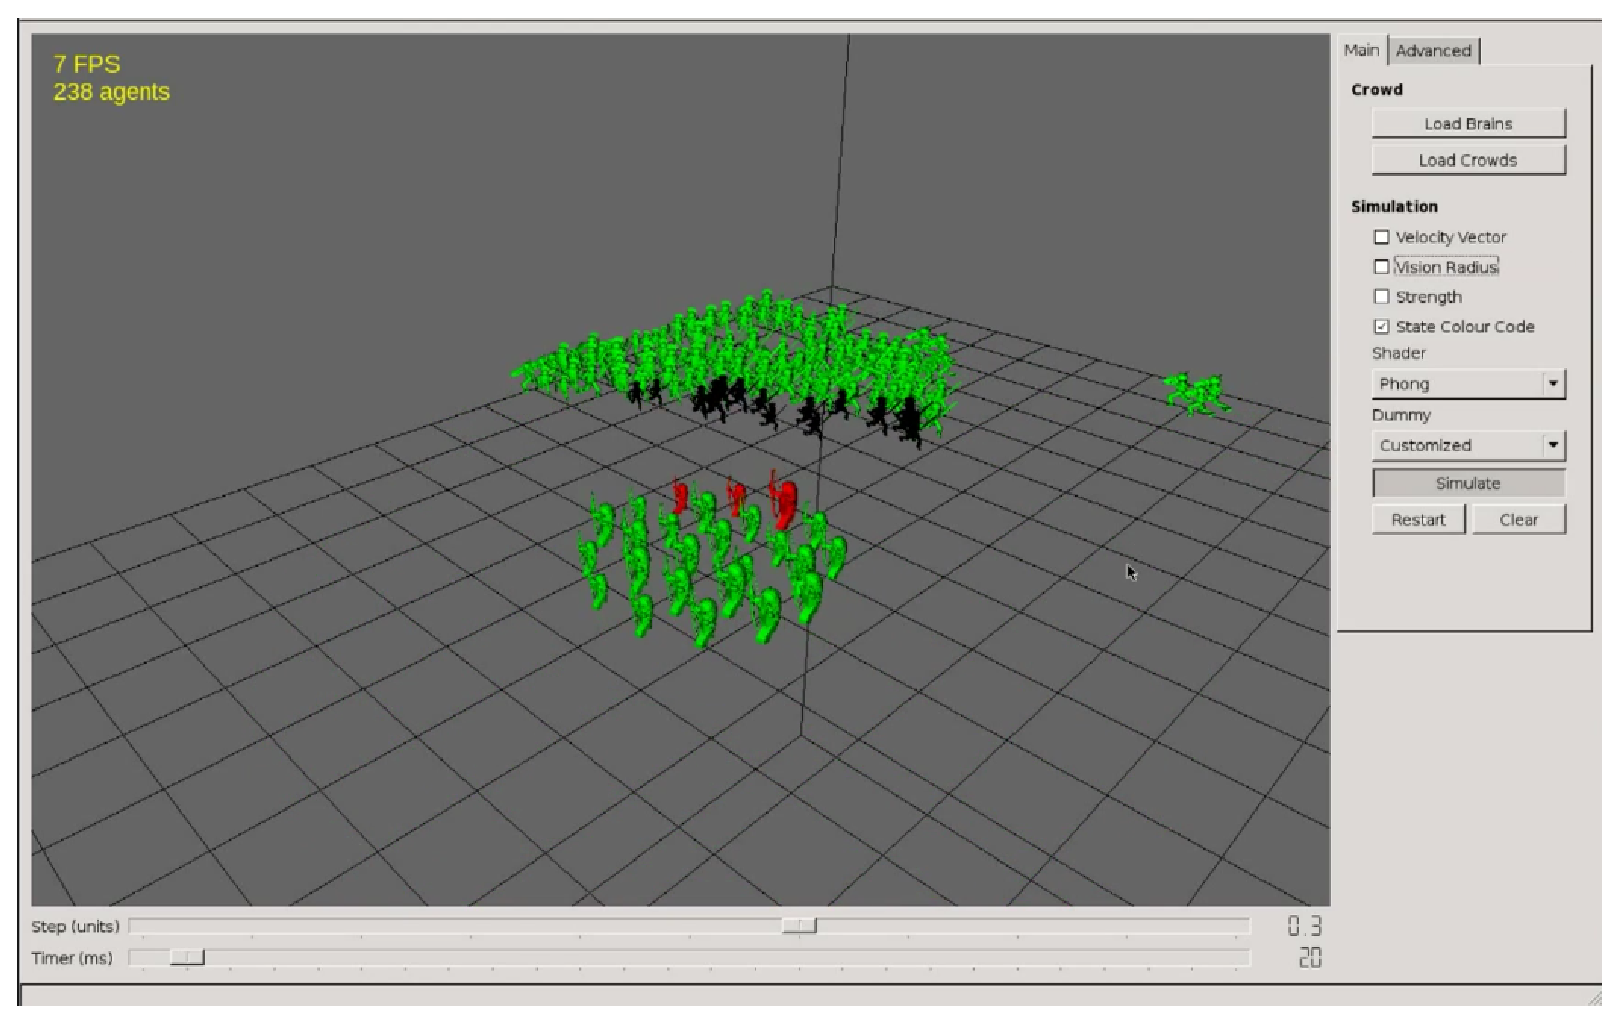
\includegraphics[scale=0.27]{archers.eps}} &
 	\subfloat[Troll behaviour]{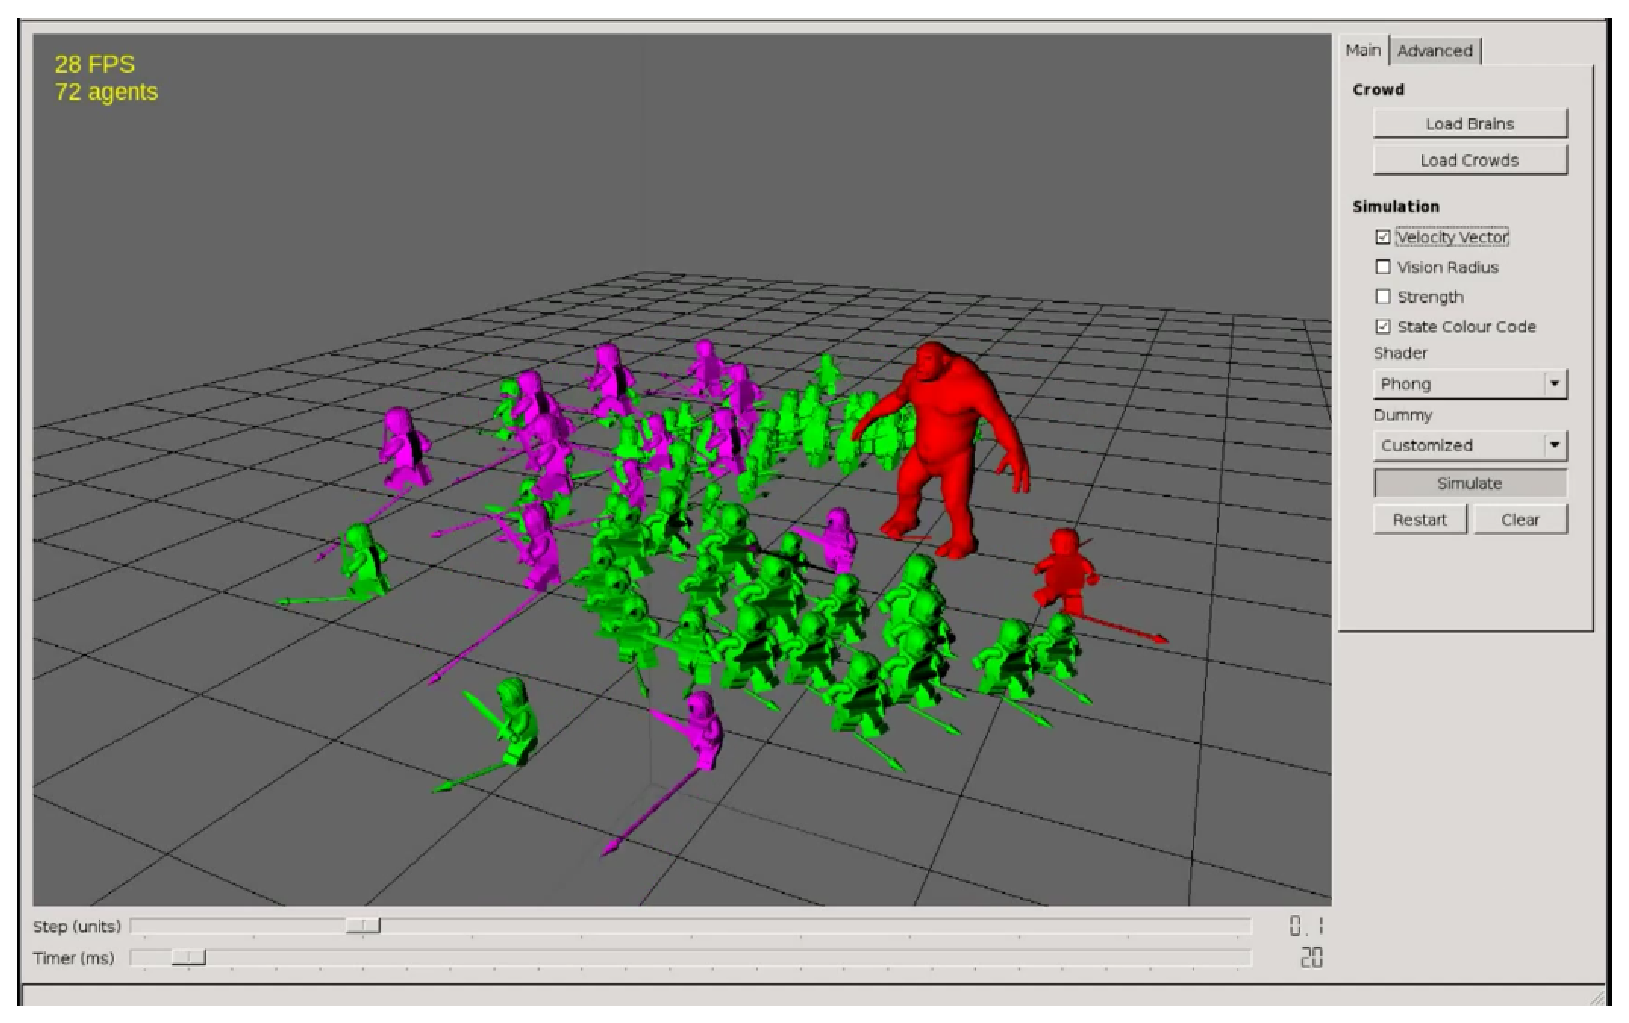
\includegraphics[scale=0.27]{troll.eps}} \\
 \end{tabular}
  \caption{Extra battle behaviours}
\end{figure}

\newpage
\subsection{A Ballroom}

To prove that not only war environments can be build with this approach, the next behaviour intends to represent A Ballroom. To achieve this, the mechanism was based in how an architecture client-server works, where the communication obtains an important role.

Firstly, we have the brain of a \emph{dancer}, which acts as a passive dancer most of the time. She is waiting in the ballroom, moving randomly. The other brain is the \emph{danceLeader}, who will find for free dancers. The protocol works in this way: the danceLeader may say ``Shall we dance?'' and the dancer will accept the request.

\begin{figure}[!h]
  \centering
  \begin{tabular}{c c}
  	\subfloat[danceLeader FSM]{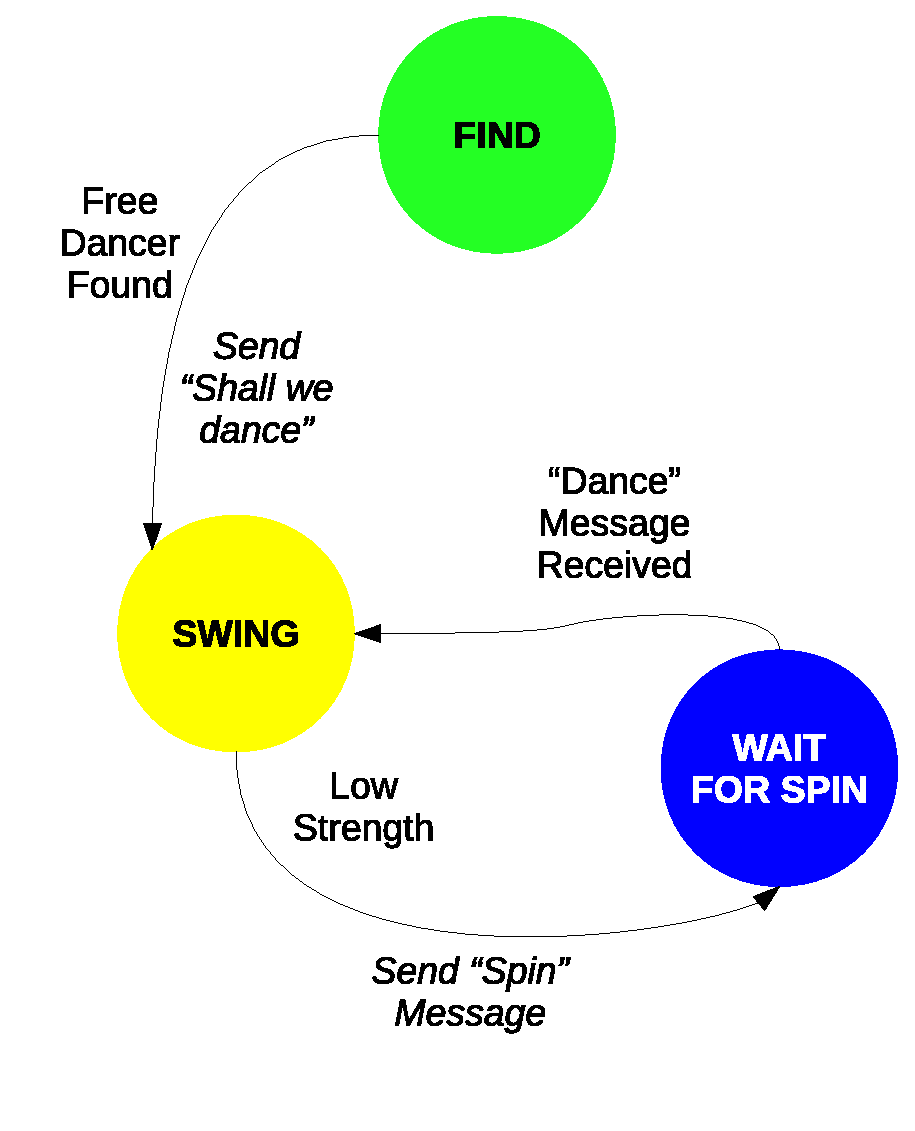
\includegraphics[scale=0.35]{danceLeaderFSM.eps}} &
 	\subfloat[dancer FSM]{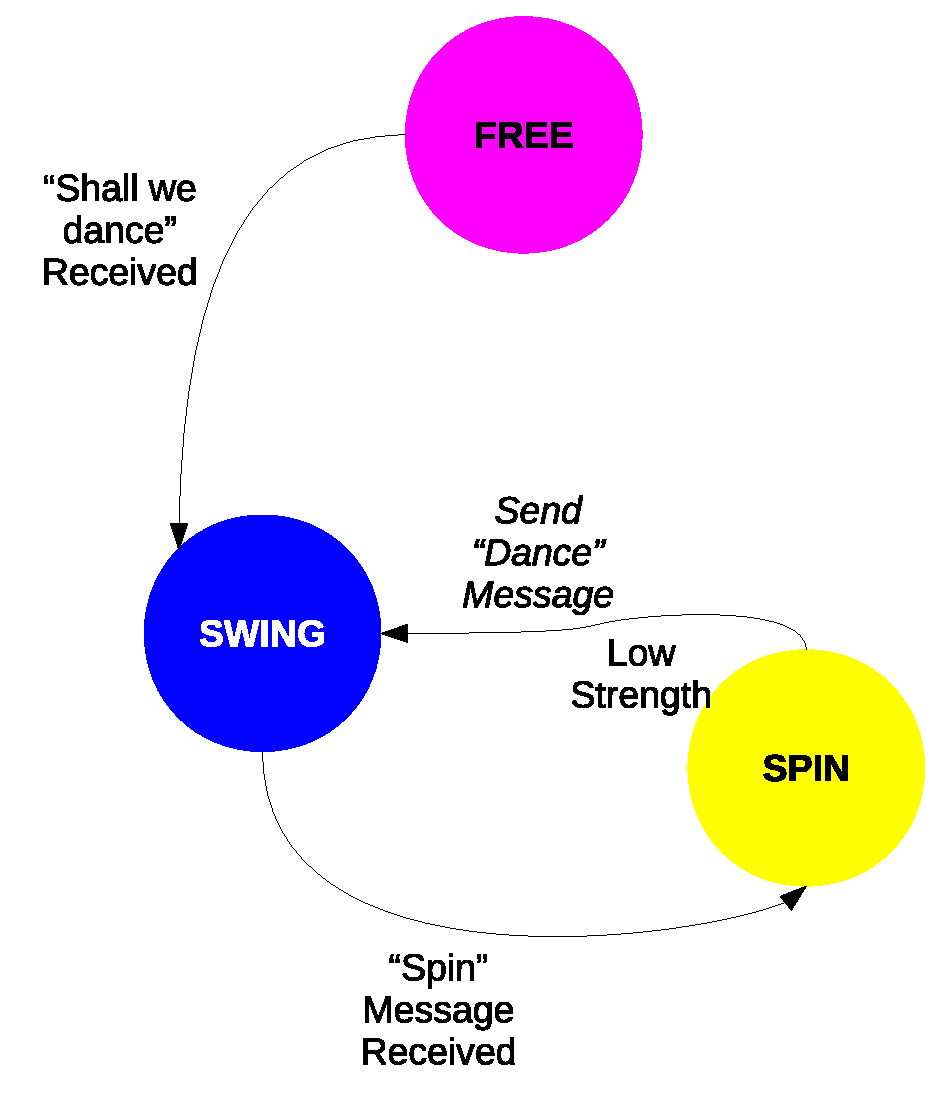
\includegraphics[scale=0.35]{dancerFSM.eps}} \\
 \end{tabular}
  \caption{FSM's for A Ballroom Simulation}
\end{figure}


The individual behaviour here may have two stages. First, danceLeaders try to find free dancers around the room and, once they find one, both start dancing together. Thus, the emergent group behaviour that can be observed here is very interesting; there will be many couples dancing and swinging graciously meanwhile some others are still finding or waiting to be found.

\begin{figure}[!h]
  \centering
  \begin{tabular}{c c}
  	\subfloat[Dancers finding partner]{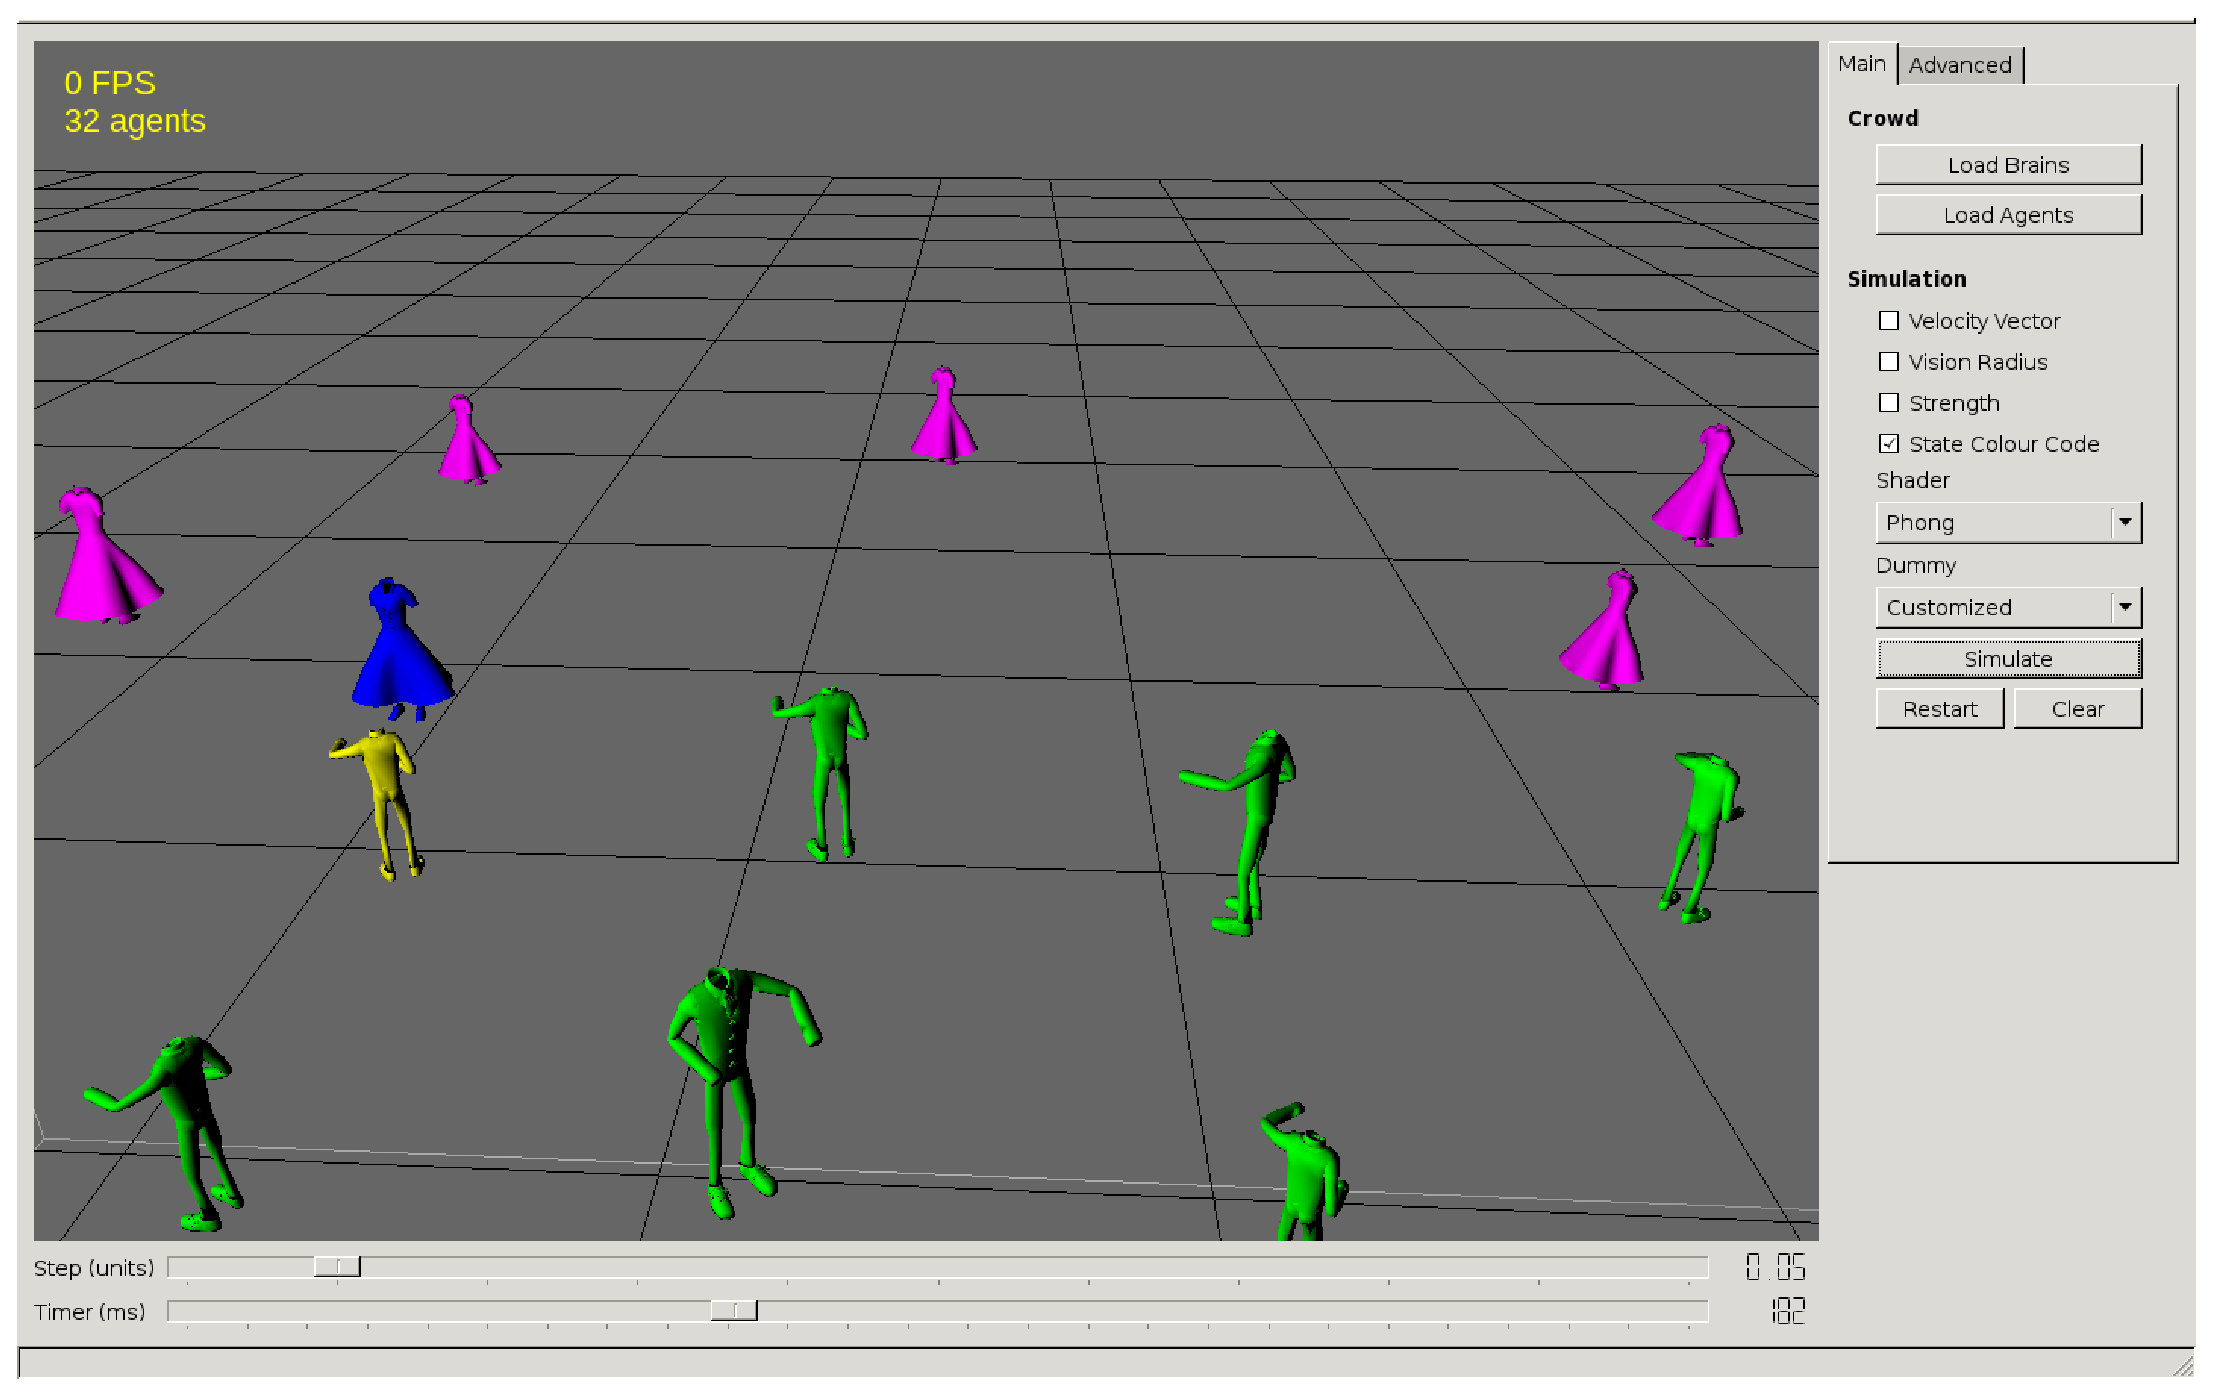
\includegraphics[scale=0.195]{ballroom_01.eps}} &
 	\subfloat[Couples swinging together]{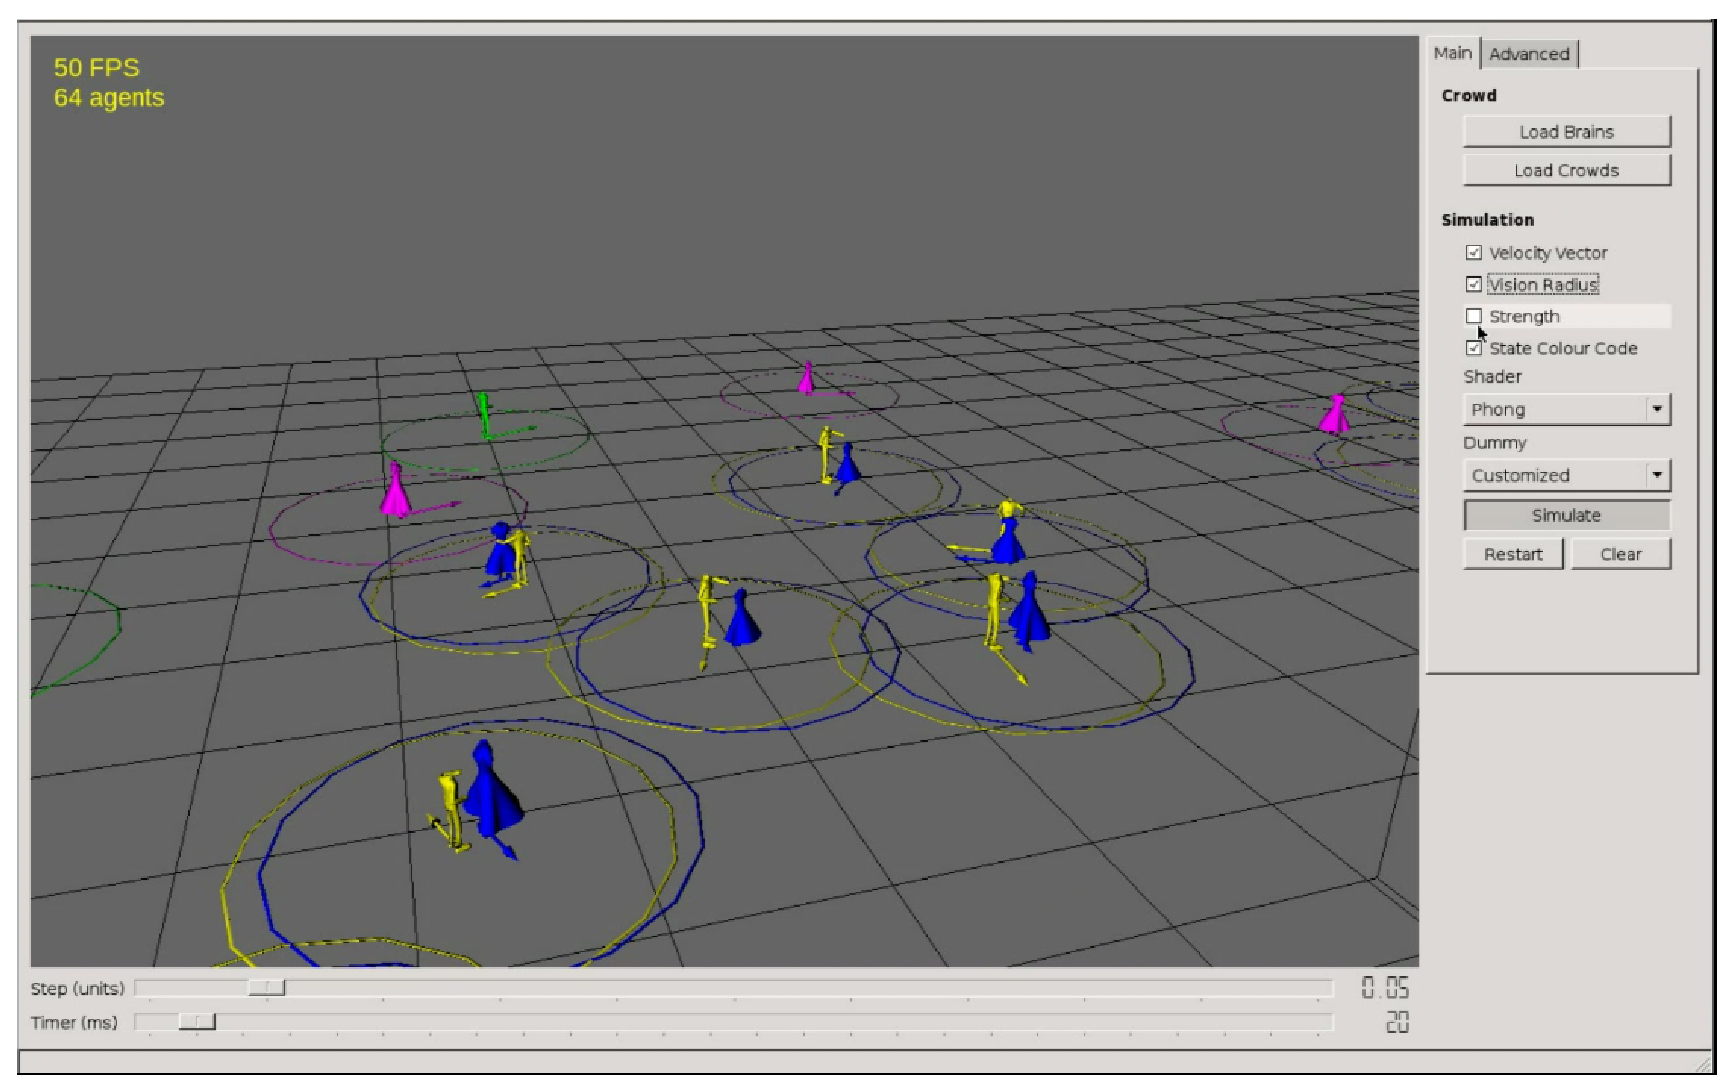
\includegraphics[scale=0.25]{ballroom_02.eps}} \\
 \end{tabular}
  \caption{A Ballroom Simulation}
  \label{fig:ballroomCaptures}
\end{figure}

\newpage
\subsection{One vs Many}

In this scenario, there is one agent who has to avoid many other agents that try to reach him. This brain was written combining forces which keep him anchored to the centre and make him attack to the incoming enemies. If this agent feels surrounded, he uses a super-attack to get rid of many enemies at the same time.

The brain of the enemies uses a simple state machine which distinguishes among the states of goingToTheMiddle, attacking and onAir. This last state allows to the enemies to know if they are in the air falling after a super attack.

\begin{figure}[!h]
  \centering
  \begin{tabular}{c c}
  	\subfloat[Blocking attacks of multiple enemies]{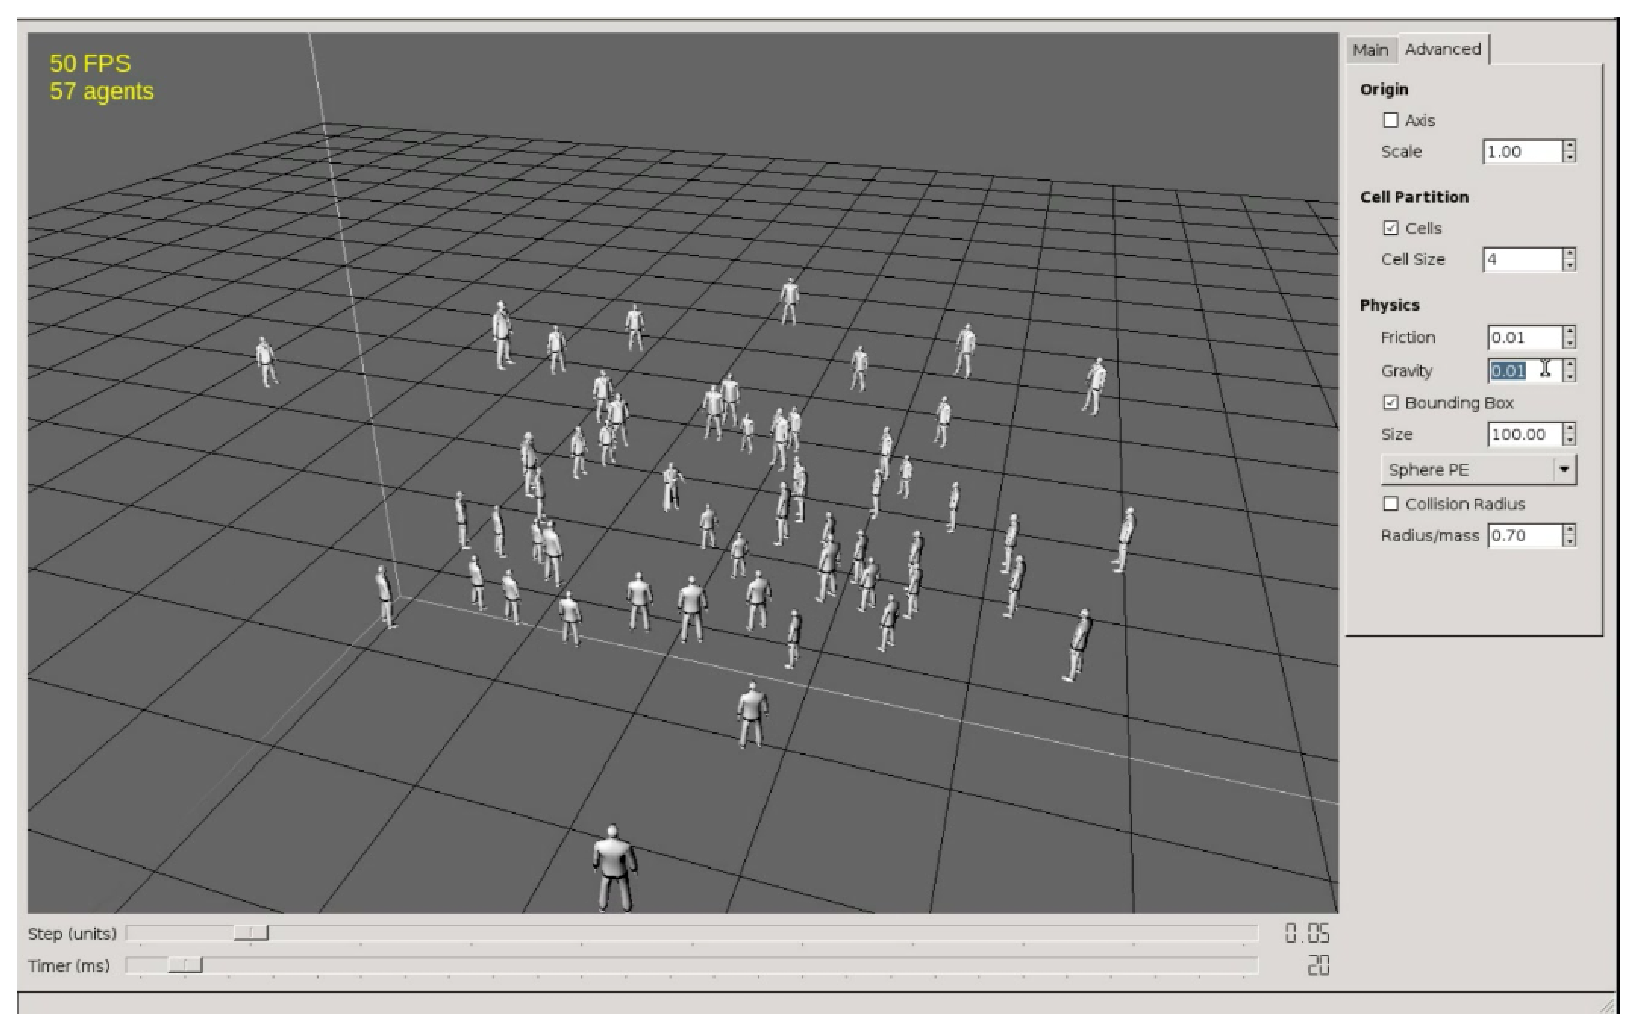
\includegraphics[scale=0.275]{matrix_01.eps}} &
 	\subfloat[Super attack to get rid of many enemies]{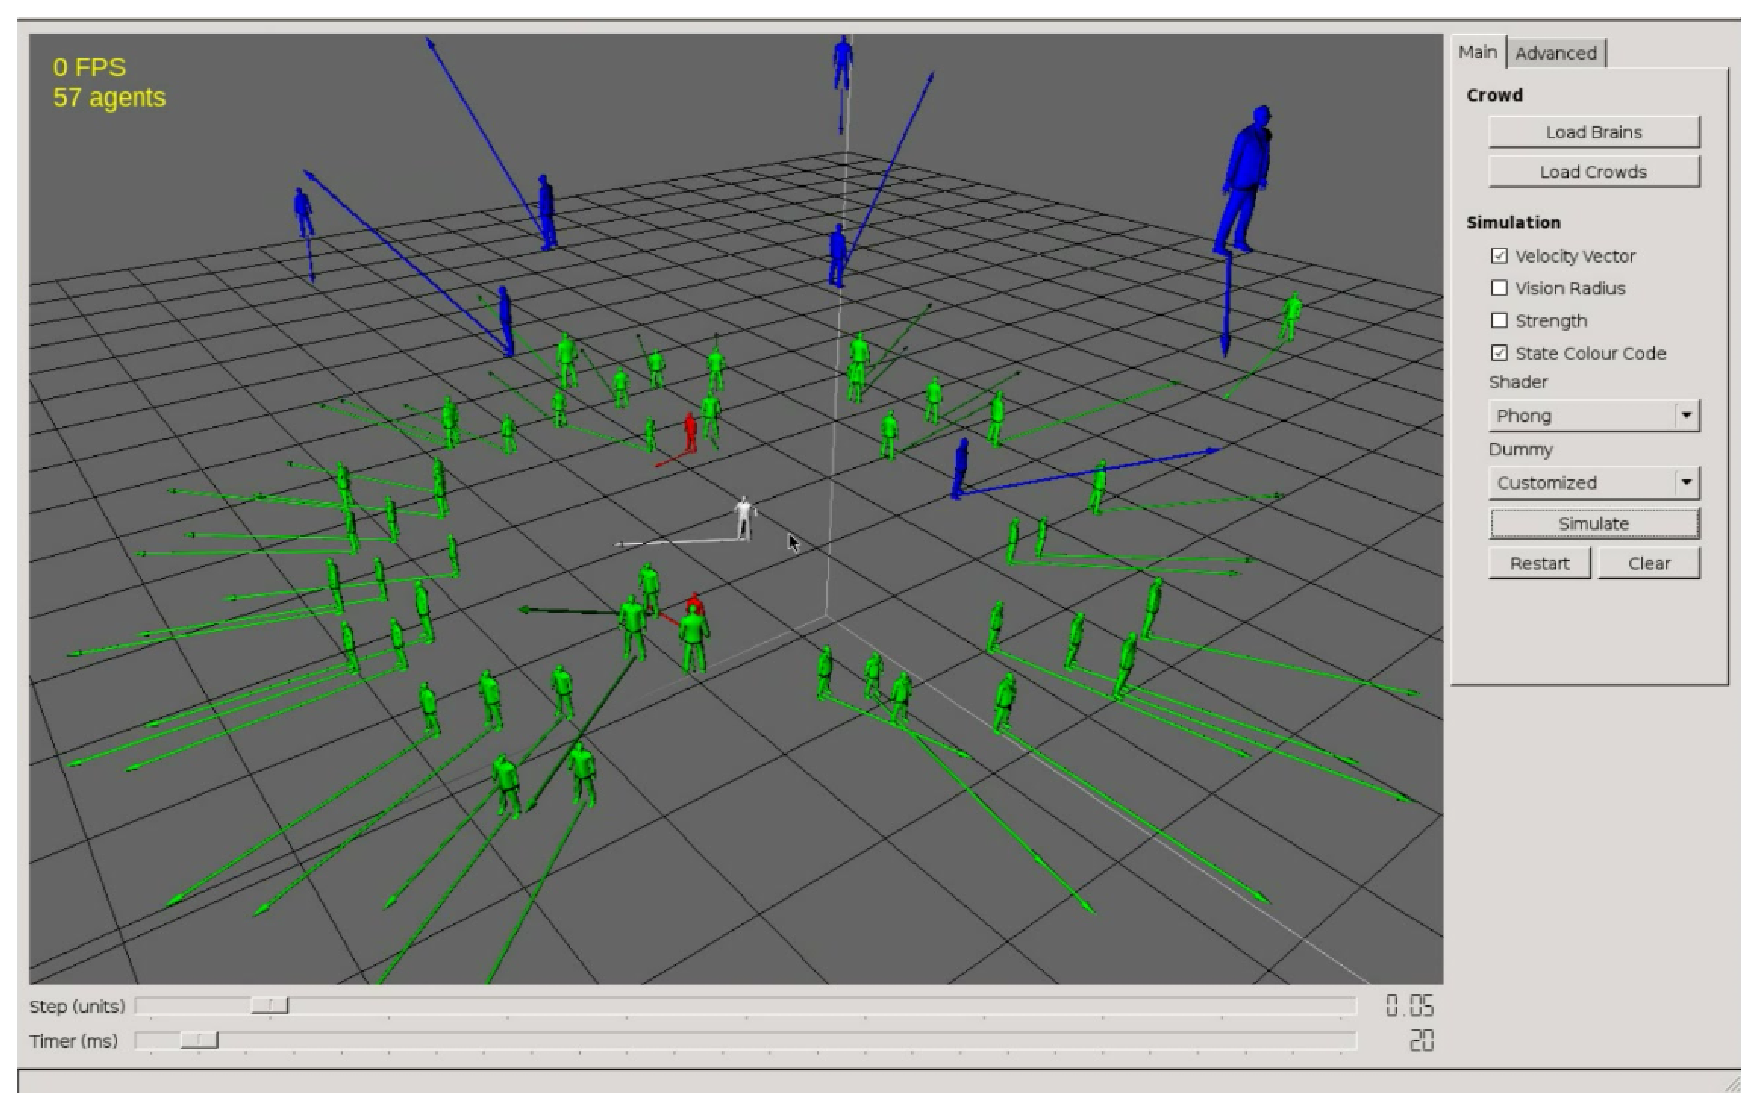
\includegraphics[scale=0.25]{matrix_02.eps}} \\
 \end{tabular}
  \caption{One vs Many Simulation}
  \label{fig:matrixCaptures}
\end{figure}

\subsection{Jumping Party}

This is another simple behaviour which includes two-state FSMs. One of the states is onFloor, which will produce an impulse to generate a jump, and the other is onAir, which works as in the last example.

\begin{figure}[!h]
  \centering
  \begin{tabular}{c c}
  	\subfloat[Jumpers' states]{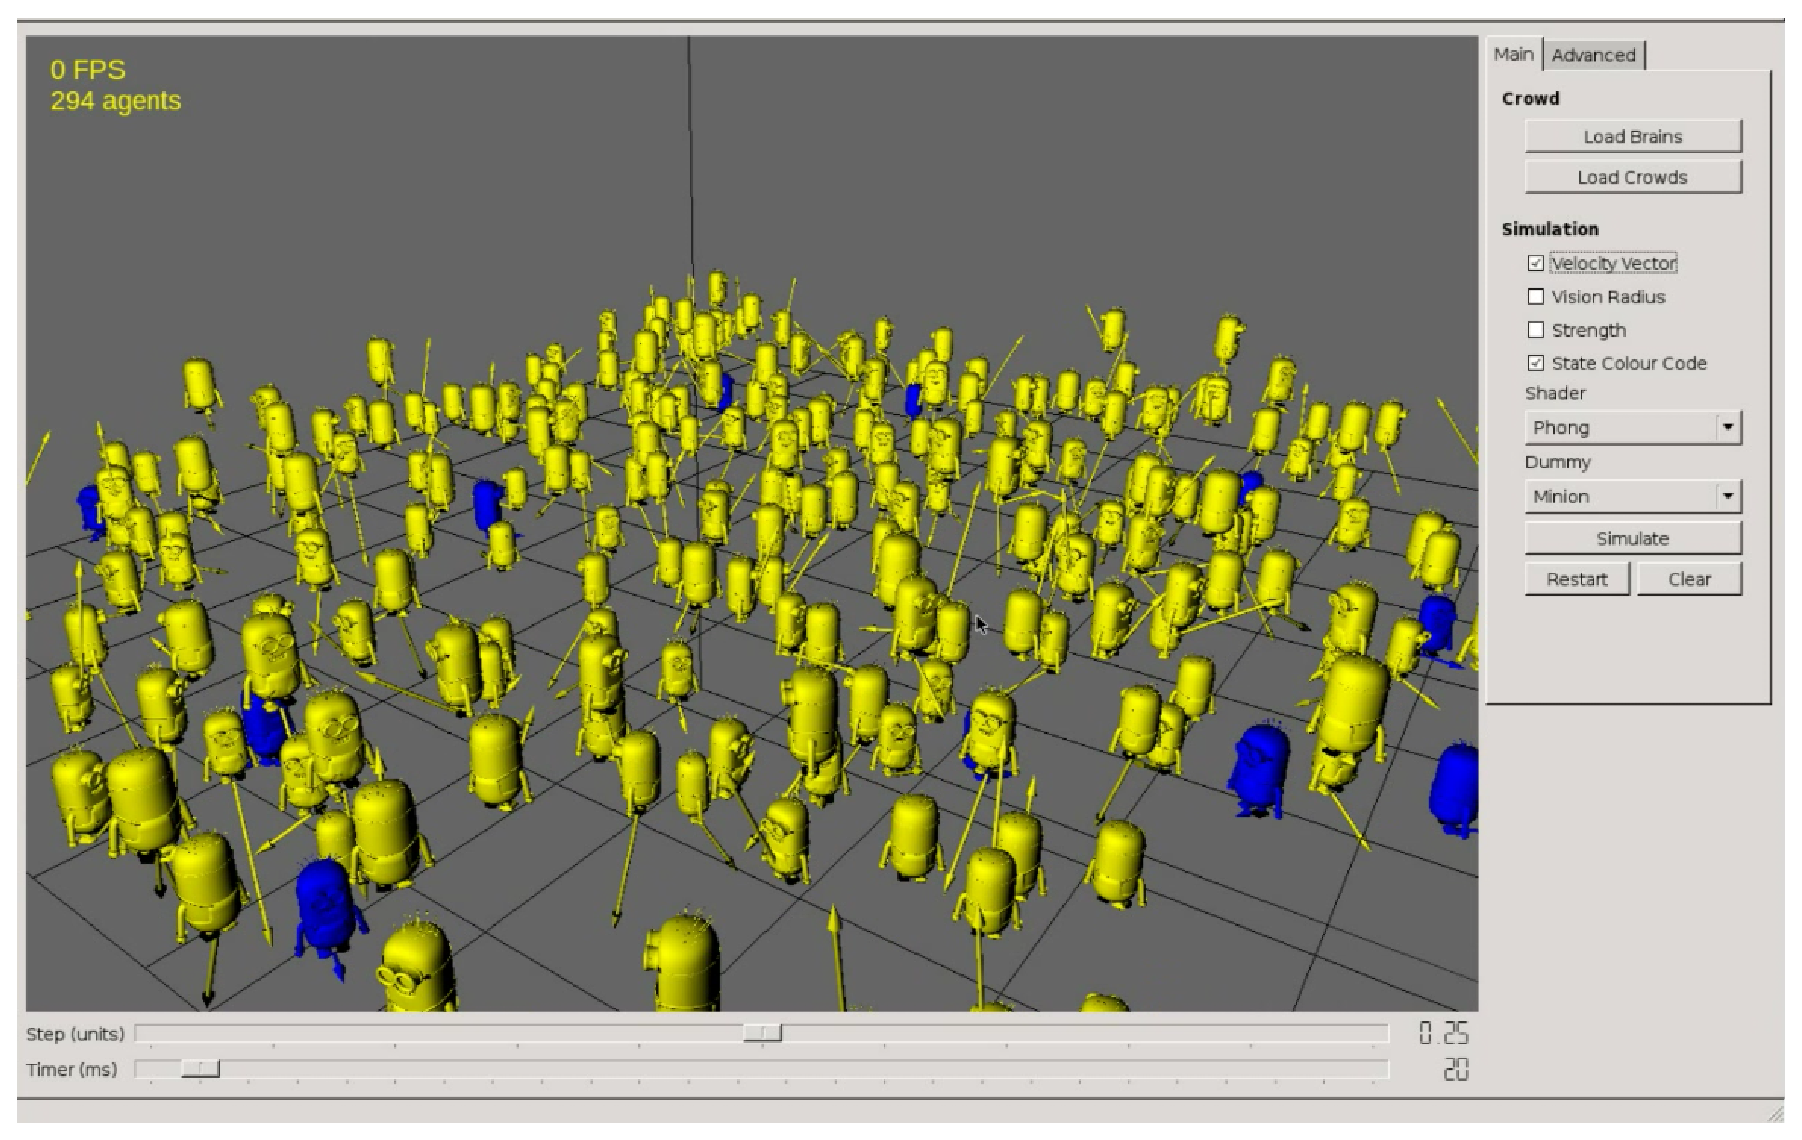
\includegraphics[scale=0.25]{minions_01.eps}} &
 	\subfloat[Jumping dummies]{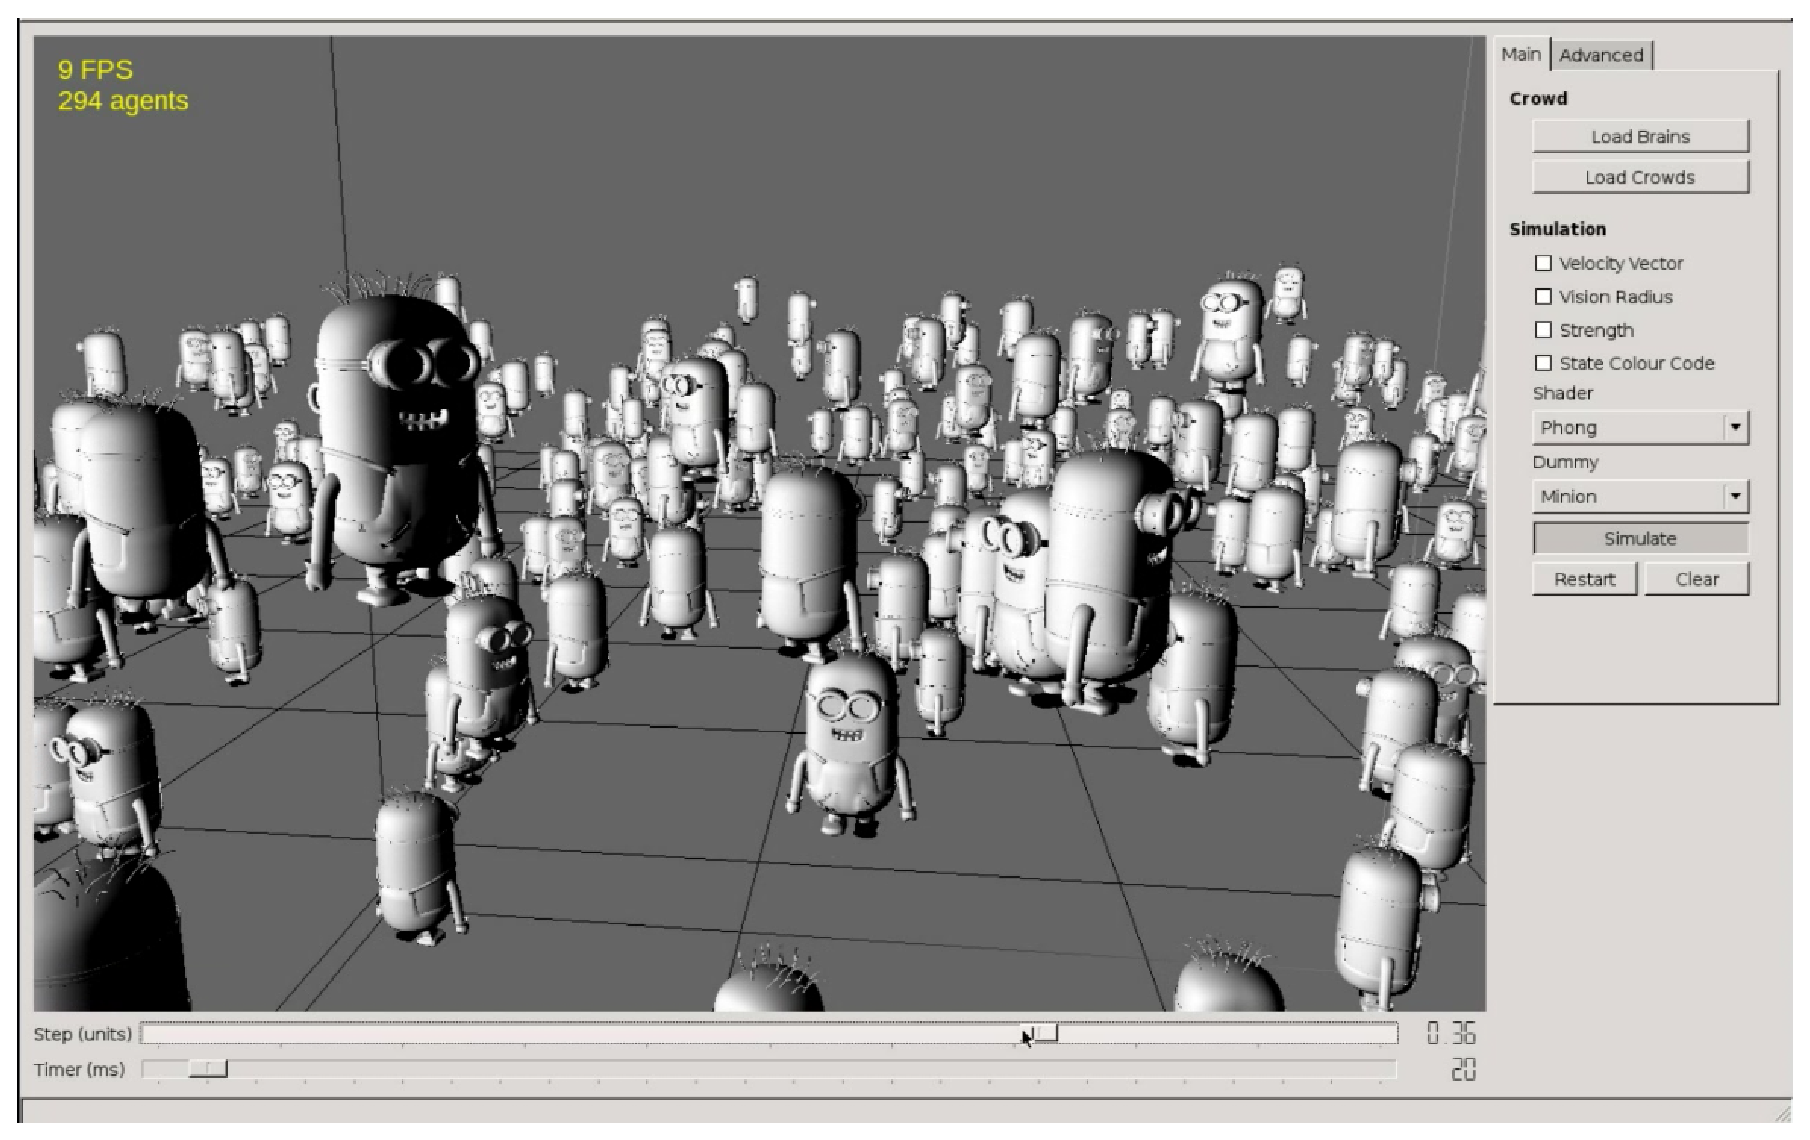
\includegraphics[scale=0.25]{minions_02.eps}} \\
 \end{tabular}
  \caption{Jumping Party Simulation}
  \label{fig:droidsCaptures}
\end{figure}


\ifx\isEmbedded\undefined
% References
\addcontentsline{toc}{chapter}{References}
\bibliographystyle{../ref/harvard}
\bibliography{../ref/master}
\pagebreak
\end{document}
\fi